\documentclass[11pt]{article}

% useful packages
\usepackage{float} 
\usepackage{fullpage} % sets more standardized margins
\usepackage{graphicx} % some graphics functions 
\usepackage{tocloft}  % single space table of contents
\usepackage[title,toc,page]{appendix}
\usepackage[nottoc]{tocbibind}
\usepackage{fancyhdr}
\usepackage{wrapfig}
\usepackage{multirow}
\usepackage{lastpage}
\usepackage{hyperref}
\usepackage{xcolor}
\usepackage{setspace}
\usepackage{titling}
\usepackage{flafter} 
\usepackage{pdfpages} 
\usepackage{titlesec}
\usepackage{rotating}
\usepackage{floatrow}
\usepackage[normalem]{ulem}
\hypersetup{
    colorlinks,
    linkcolor={red!55!black},
    citecolor={blue!50!black},
    urlcolor={blue!80!black}
}

% to comport to IEEE style for referencing figures
\usepackage[justification=centering]{caption}
\usepackage[figurename=Fig.]{caption}
\captionsetup{labelsep = period}
%\captionsetup[table]{labelsep=newline}
%\captionsetup[table]{name=TABLE}
%\renewcommand{\thetable}{\Roman{table}}
\captionsetup[figure]{labelsep=period}

% paragraph indentation and separation
\parindent = 0.0in  
\parskip = 12pt
%\renewcommand{\absnamepos}{flushleft} % left justifies abstract

% use Arial font
%\usepackage{fontspec}
%\setmainfont{Arial}

% header and footer
\renewcommand{\headrulewidth}{0.0pt}
\renewcommand{\footrulewidth}{0.4pt}
\lfoot{{\fontsize{10}{11} \selectfont ECE 403 - Capstone Project Report}}
\cfoot{}
\rfoot{\fontsize{10}{11} \selectfont \thepage\ of \pageref{LastPage}}
\lhead{}
\chead{}
\rhead{}
\pagestyle{fancy}


%\documentclass{titlepage}% use option titlepage to get the title on a page of its own.
\begin{document}
% blindtext looks like a "lorem ipsum" generator, which we definitely don't need
%\usepackage{blindtext}
% Title and author
\title{ \textbf{Fort Score, and Sixty Years Ago: A Time Machine}}
%\title{ \textbf{Vintage Scoreboard with Digital and Analog Clocks}}
\author{Ally DiFilippo \\
Miles Martin\\ \\
University of Maine \\
ECE 403 Project Report}
\date{\today}
\maketitle
\thispagestyle{empty}
\pagenumbering{roman}




\newpage

%\begin{document}

% Abstract 
\begin{center}
\section*{Abstract}
\end{center}
\noindent
This report details the process of overhauling and repurposing a vintage basketball scoreboard belonging to the town of Fort Fairfield, ME. 
The clock face that previously was an 8-minute timer for basketball periods was to be turned into a 12-hour analog clock. 
Additionally, the score-keeping display's functionality was to be replaced with that of a digital clock.
The incandescent light bulbs were replaced with LED-based light bulbs as a long-term substitute. The device is powered from a 120 V$_{rms}$ wall outlet. 
An on-board Raspberry Pi (RPi) creates and manages an intranet website hosting a Graphical User Interface (GUI). 
% The RPi facilitates the collection and parsing of GUI input using a wireless network connection. 
A wireless network connection to the RPi facilitates the collection and parsing of GUI input. 
User input is transmitted through a Universal Asynchronous Receiver and Transmitter (UART) serial connection to the microcontroller, and the input is used for motor control.
The motor control microcontroller uses a virtual serial port to forward time data via UART to the LED matrix driver's microcontroller.
Each clock control microcontroller parses the time data, and displays the appropriate time. The device uses Network Time Protocol (NTP) to ensure accuracy to  Coordinated Universal Time (UTC) which then is used for the system time based on the time zone set. 
User input allows the current clock display time to be overridden as well as other control functions. 



\newpage
\tableofcontents


\newpage
\listoffigures
\listoftables


\newpage 
\pagenumbering{arabic} % Turn on page numbering


%The purpose of the introduction is to contextualize your project for a general audience.  The introduction should be a clear overall discussion of the project in broad general terms.  Describe the project in simple terms that a lay person who does not have a technical degree could understand.  Specifically, explain the purpose, background, context, and overall operation of the project.  Describe why you chose to build this project.  Explain the specifications and terms of the contract.  Briefly describe how specifications were verified.  Compare your project with other similar devices. Discuss any other matters that will help the reader understand the purpose of your project.  Add other background information that will make the rest of the report easier to understand. 

% Introduction section
\section{Introduction}

This document describes the design and testing of the repurposing of a vintage basketball scoreboard to have analog and digital clock functionality for the Recreation Department of Fort Fairfield, Maine.
Constant advancements in the field of electronics have shortened the time between the release and obsolescence of new technology, creating an influx in technological waste. 
It is the antithesis of that concept which drives this project: a strong focus on repurposing and understanding the hardware of the past has prevented greater wastefulness.
The client and sponsor of this project, the Recreation Department of Fort Fairfield, ME, had recently acquired a new modern scoreboard. 
It was the client's thoughtfulness that led to re-envisioning this vintage scoreboard as an analog and digital clock, which is where this project begins.
%which provides the basis for this project.
% Talk about specs here 
% I tried to figure out how to do the lettered appendix but this was the best lead I could find: https://tex.stackexchange.com/questions/174621/numbering-appendices-by-letter-instead-of-number https://www.overleaf.com/project/61f15cf67f52669e734513b3
The specifications for this project are outlined in the project contract found in Appendix \ref{appendix:contract}. 

%Nuri said he wanted these in prose in the rubric
% \begin{itemize}
%     \setlength\itemsep{0.2em}
%     \renewcommand\labelitemi{--} % This decides the format of the bullet points.
%     \item User input must be able to be able to control/program the clock. 
%     \item The scoreboard must be controlled by a Raspberry Pi single-board computer. 
%     \item The time display on both the analog and digital clock must have accuracy to the minute. 
% \end{itemize}

These specifications can be summarized as three main constraints. First, the device's input consists of power being supplied from a 120 $V_{rms}$ wall outlet and user input through a GUI that must be able to control/program the clock. Second, the project itself must be controlled by a Raspberry Pi single-board computer, and have networking capability via Wi-Fi. Finally, the output of the project should be the visual display of the analog and digital clock with accuracy to the minute. 


%flagging this, I don't like the first dependent clause
%While not a written specification here, 
In addition to these specifications, the design process was carried out with a desire to preserve as much of the scoreboard's original hardware as possible. 
The unique history of this piece as an antique presented physical and mechanical constraints that were addressed throughout the project. 
While the primary goal of this project was to return this piece of history to service, the complication of maintaining its historical value while incorporating modern technology was a consideration constantly balanced by the team.
%presented difficulties throughout the entire process. 
% .

%flagging this, I don't like it because it's really wordy/long
% Certain parts of the scoreboard being custom made and made several decades ago led to difficulties in the procurement of replacement parts given the necessity to avoid replacing any external parts of the board to preserve its history, and requiring creative and unconventional approaches to aspects of the design. 
The scoreboard's fabricators used what would now be considered antiquated electronic design and small-scale- or traditional manufacturing techniques.
These design choices on the part of the original scoreboard engineers guided those of the overhaul team.
For example, irreplaceable and otherwise old parts of the vintage design made the redesign process more difficult.
The methods by which some of the scoreboard's parts were machined and produced, in addition to the age of these parts, makes it difficult for the team to replace some original hardware.
Therefore, the replacement of external parts on the scoreboard was limited to the lenses over the digital clock display, with the added possibility of other out-of-sight locations. 
%Certain parts of the scoreboard being custom made and made several decades ago led to difficulties in the procurement of replacement parts given the necessity to avoid replacing any external parts of the board to preserve its history, and requiring creative and unconventional approaches to aspects of the design.
This stipulation is important because internal access to the unit is very limited, causing replacing and mounting of internal equipment to be more difficult. 
In addition, the unit will be installed in a high-traffic recreational area, so durability and stability were additional concerns for this redesign.
% other intro paragraphs above this final paragraph

The process of designing and constructing each part of this project is described throughout this report. 
Section (\ref{breakdown}) provides a breakdown of the project, including functional block diagrams and an overall discussion of the system functionality. 
Section (\ref{details}) provides more in-depth details of the design, including a closer look at the hardware and software design structure, and how data is transmitted through the various components. 
Section (\ref{results}) discusses the results of the project while Section (\ref{conclusion}) is a conclusion. 


\section{Project Breakdown}
\label{breakdown}
% Block diagram
% Explain in subsections what the parts of the block diagram are, block by block, including inputs, outputs, and transformations occurring therein
This section documents a high level overview of the major functional components of the scoreboard device. 
Similarly, block diagrams of the hardware and software aspects of the project will also be discussed. 
The overall project block diagram can be seen in Figure \ref{OverallBlock}.

The scoreboard clock project consists of four primary blocks: Power Management, Motor Control, LED Matrix Control, and an Intranet Web Server. 

\begin{figure}[H]
\centering
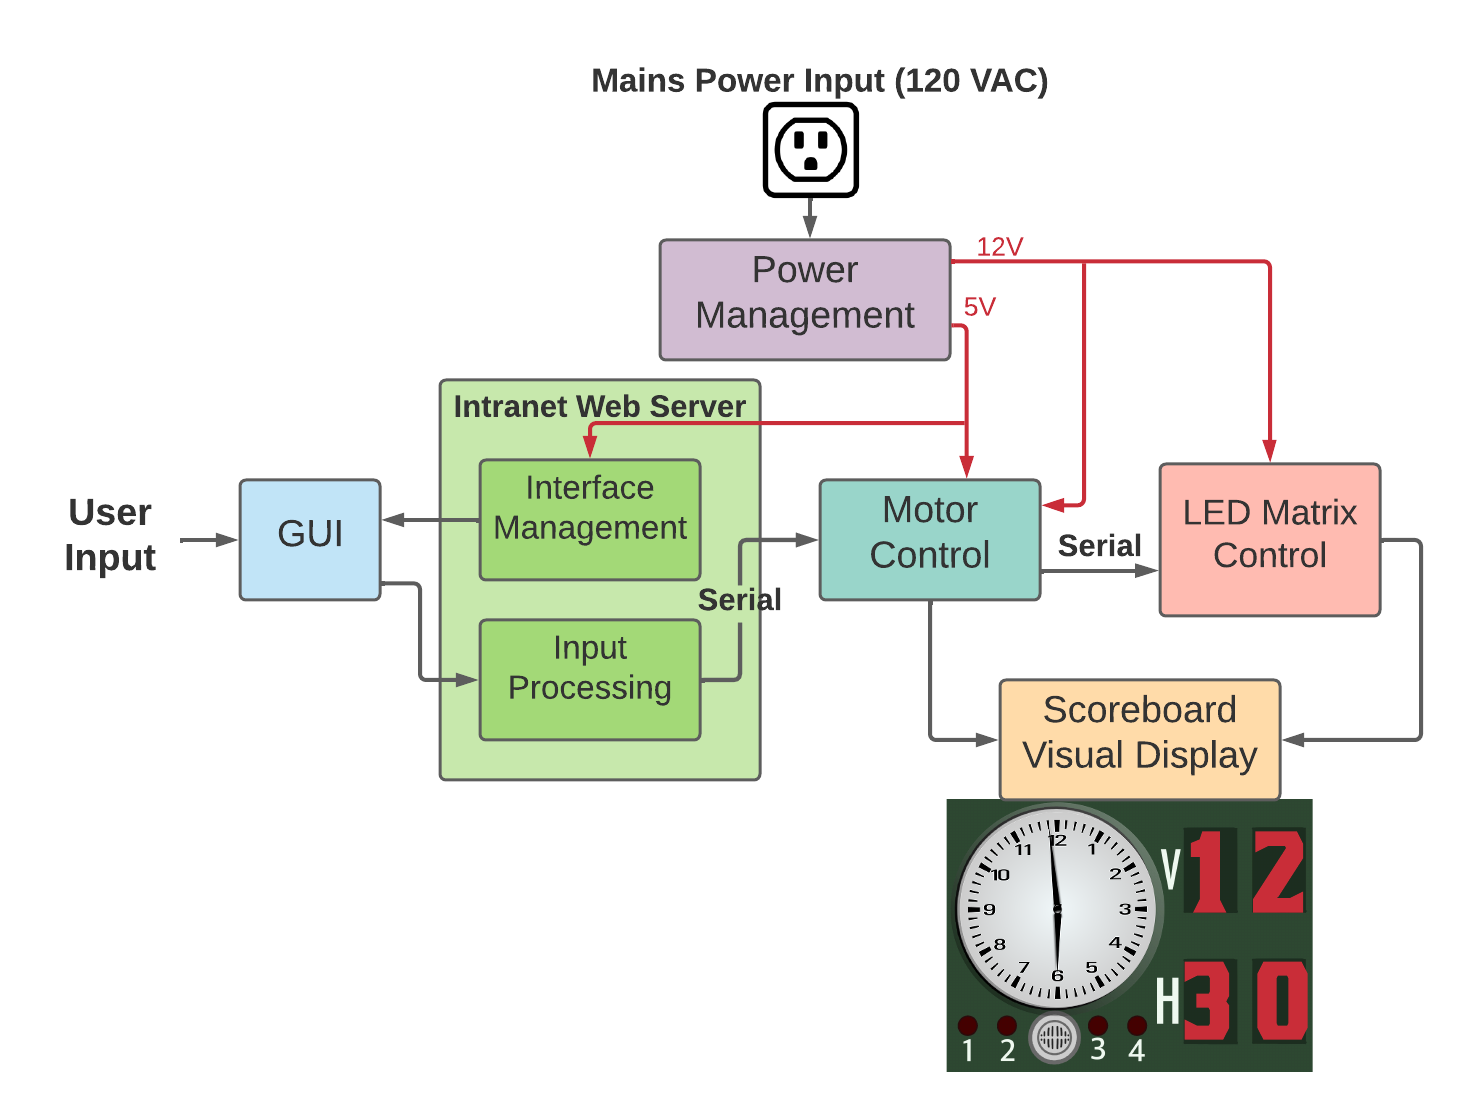
\includegraphics[width=6in]{Functional_Block_Diagram.png}
\caption{Simplified Block Diagram of Scoreboard with Digital and Analog Clocks}
\label{OverallBlock}
\end{figure}

%Power management is illustrated further in Figure \ref{PowerBlock} of Section \ref{HardBreakdown}.
Details of the power management system are found in Figure \ref{PowerBlock} of Section \ref{HardBreakdown}.
A Graphical User Interface (GUI) managed by the Intranet Web Server (a \textbf{Python}-based Flask framework) receives User Input. 
Input is provided through an HTML webpage, and an Intranet Web Server outputs times. 

An overview of the project with a focus on the software aspects designed, including the Intranet Web Server, can be found in Section \ref{SoftBreakdown} with Figure \ref{SoftBlock}. 
The software of the motor control and LED matrix control, as well as the serial communications that provides controls for both, are broken down further in Figure \ref{SerialBlock}.

\subsection{Hardware Breakdown}
\label{HardBreakdown}

%The design of the scoreboard project had a heavy dependence on hardware and mechanical elements. 
The technical debt of inheriting the scoreboard's chassis provided a unique set of design challenges and considerations throughout the project. 
The ways in which the mechanical components impacted the design process will be discussed in Section \ref{details}. 

The hardware of the project consists of four main parts: the Raspberry Pi, the microcontroller boards, the Motor Control circuitry, and the LED Matrix Control circuitry. 
The Raspberry Pi handles the user interface and input processing, as will be discussed in more detail in Section \ref{SoftBreakdown}. 
The ATmega board, a clone of the Arduino Mega microcontroller, is responsible for controlling the input signals to the drivers of the motors.
Additionally, it reads the output from the continuous rotary encoders. 
It also forwards the serial input it received from the Raspberry Pi to a Texas Instruments Tiva C-Series board, using the UART protocol. 
The Tiva board is responsible for processing that serial input signal and controlling the input signals to the LED Matrix control PCBs. 
The motors and LED Matrices, according the received signals, then display the analog and digital time respectively through movement of clock hands and lighting of corresponding LEDs.  

%The following subsection will focus on providing a breakdown of the power management of the device specifically. 

\subsubsection{Power Management}
% TODO (MILES)


\label{PowerBreakdown}

An overview of the path of power through the project can be seen in Figure \ref{PowerBlock}. 

\begin{figure}[H]
\centering
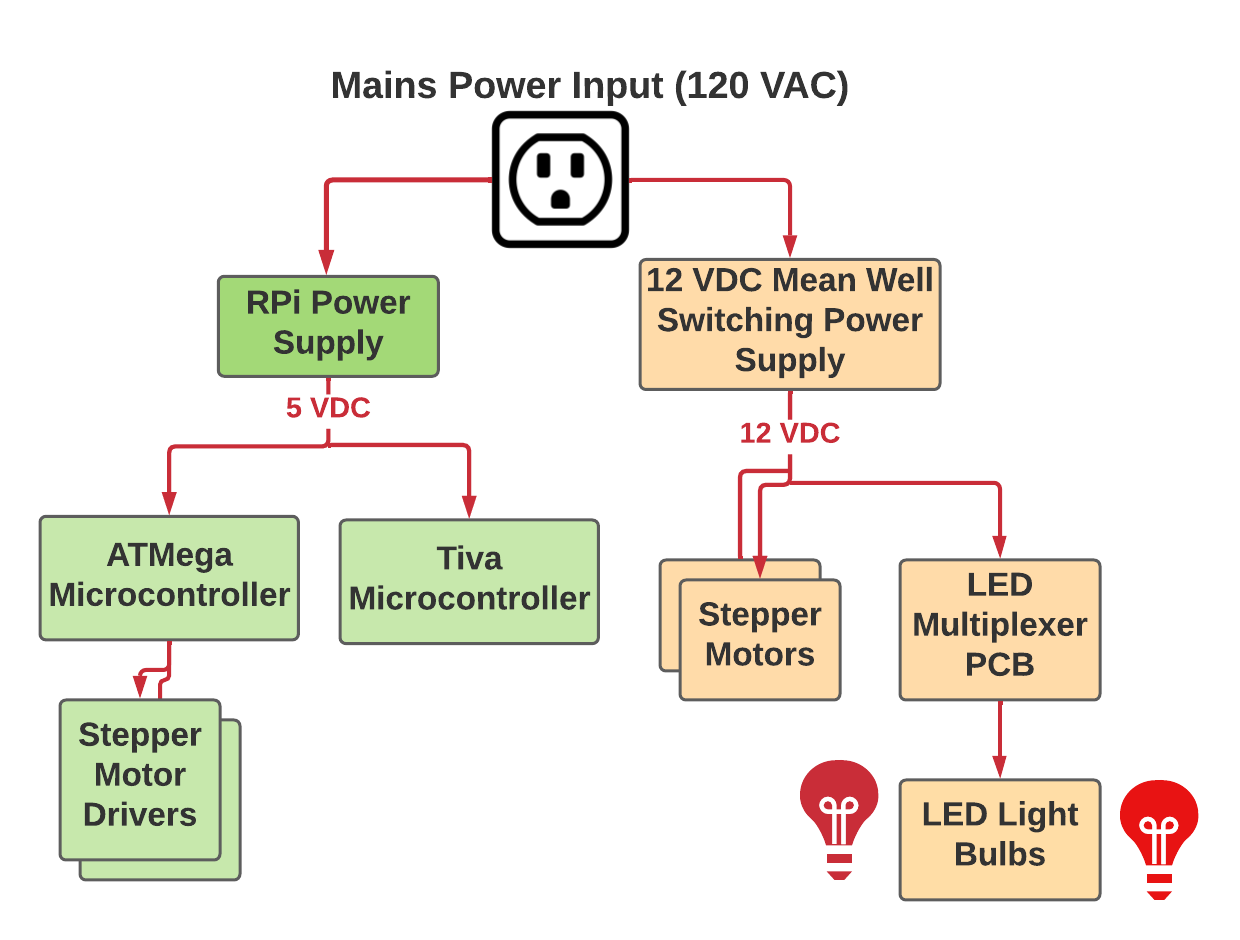
\includegraphics[width=4.5in]{Power_Diagram.png}
\caption{Power Management Block Diagram of Scoreboard with Digital and Analog Clocks }
\label{PowerBlock}
\end{figure}
Power is provided to the device through its input, a NEMA 5-15 extension cord. 
Single-phase power supplied at 120 $V_{rms}$ using either NEMA 5-15 or NEMA 1-15 wiring, plugs, receptacles, or sockets will be herein referred to as "mains power".
Internally, the end of the extension cord is used to power two  AC-DC power supplies through a repurposed set of wall-outlet strips. 

A Raspberry Pi 15 W Power Supply (the official and recommended power supply unit (PSU)) takes an AC input of 120 $V_{rms}$ and supplies 5.1 VDC at up to 3 A to the RPi.
Additionally, a Mean Well RS-15-12 unit uses mains power to  supply 12 VDC at up to 1.3 A, totaling 15 W.
The Mean Well supply provides the power that runs the Scoreboard Visual Display. 
12VDC is supplied to each of the two stepper motors that move the analog clock hands, as well as power to the LED multiplexer PCB that drives the digital clock display.
The ATmega and Tiva boards also require power at 5 VDC, which can be provided by the Raspberry Pi, supplied over USB.
The two stepper motor drivers used also required 5 VDC, which was provided through a connection to the ATmega board. 





\subsection{Software Breakdown}
\label{SoftBreakdown}

% Awkward wording, reword
The software of this project has two main parts: The \textbf{Flask} Web Server \& GUI, and the Microcontrollers that control the hardware. A block diagram providing an overview of the software can be seen in Figure \ref{SoftBlock}.

\begin{figure}[H]
\centering
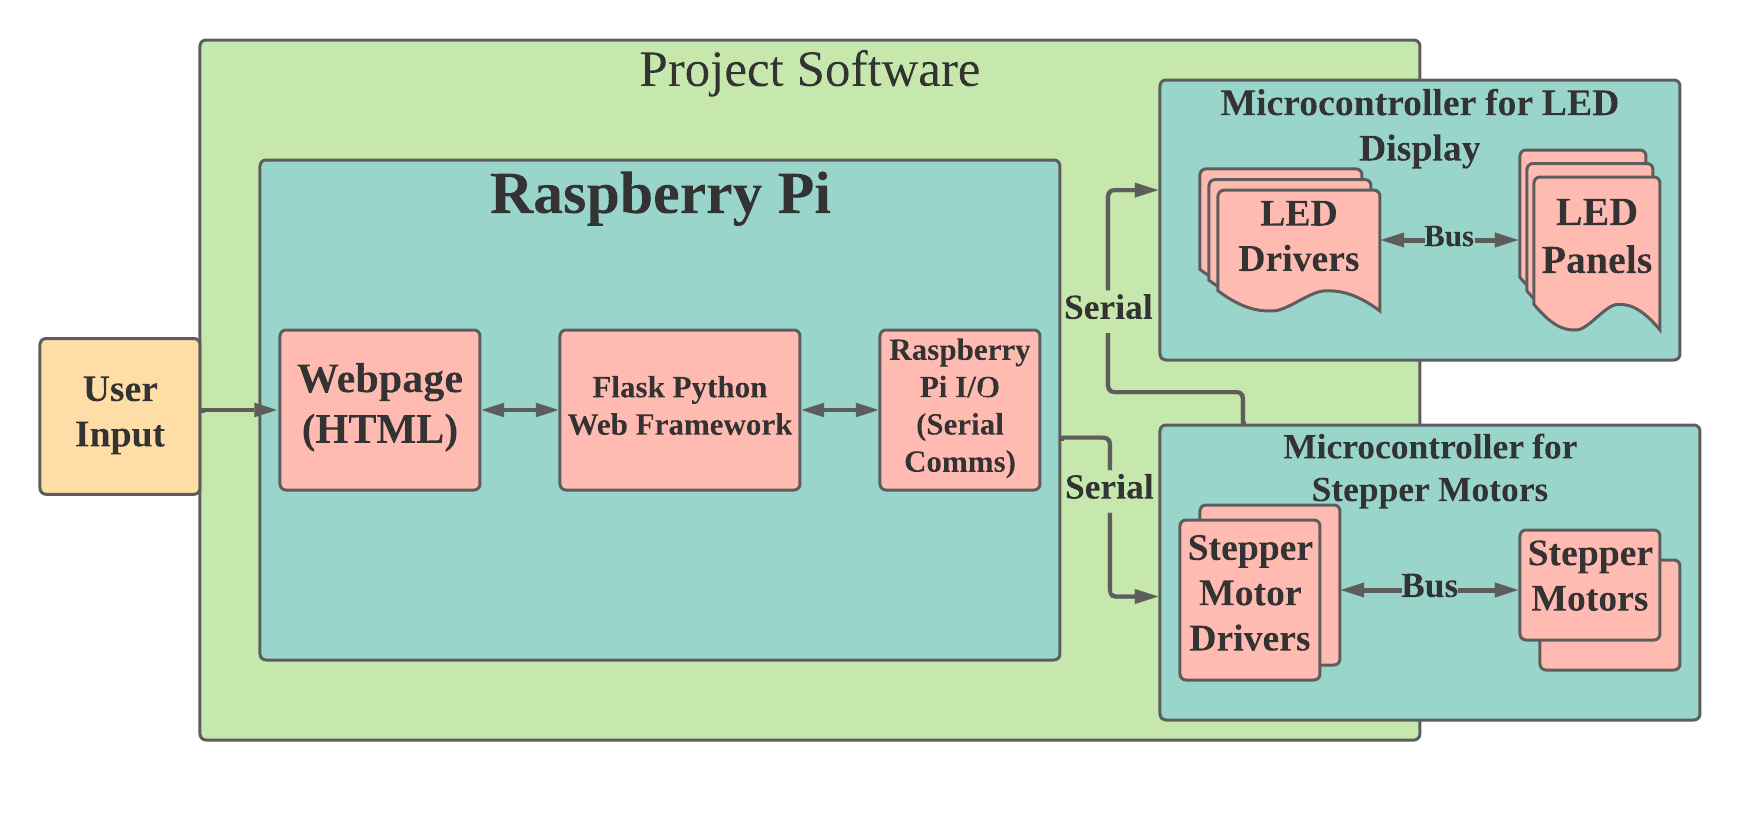
\includegraphics[width=6in]{Software_Nema_7.png}
\caption{Software Block Diagram of Scoreboard with Digital and Analog Clocks }
\label{SoftBlock}
\end{figure}

As can be seen in Figure \ref{SoftBlock}, the Raspberry Pi is responsible for software that runs the \textbf{Flask} Web Server that controls the GUI and receives and parses user input that then sends the input for the ATmega microcontroller over serial. 
 

\subsubsection{Flask Web Framework}
\label{FlaskBreakdown}

% Runs GUI, gets \textbf{datetime}, takes user input, formats it and sends it over serial

\textbf{Flask} is a \textbf{Python}-based web microframework. 
In this context, a microframework is one that does not provide form validation, database abstraction, or similar functionality that can be provided by a library. 
It is a framework built with the intent to support extensions with ease to provide the necessary functionality without unnecessary bloat that comes with other general-purpose frameworks. 

A \textbf{Flask} web framework was designed to provide the GUI as an HTML template capable of receiving and prompting user input, as well as fetch the RTC current time, and parse user input into the desired format and sending it over serial communications to the ATmega microcontroller board. 

The GUI accepts user input as a form on an HTML webpage run by the \textbf{Flask} framework. 
It allows for multiple user options of resetting the time to a "zero" from the rotary encoders, indicating noon, based on either the hardware or software "zero" position of the rotary encoder.
This essentially allows for adjustment of the clock to the proper time even if, over the course of the project's life, the accuracy of the rotary encoder changes. 
Similarly, another user option is submitting the exact time the user wishes to display, and the clock will proceed to tick forward from that time.
While the usage of the GUI requires an internet connection, the microcontrollers, after an initial receiving input, can continue to update and display time without continued input, allowing the clock's time to remain accurate even without continued internet access. 

\subsubsection{Microcontrollers}
\label{MicroBreakdown}

Each microcontroller receives serial input in the format of a string indicating the desired action and time for the display. 
This system of serial communication is illustrated in Figure \ref{SerialBlock}.

\begin{figure}[H]
\centering
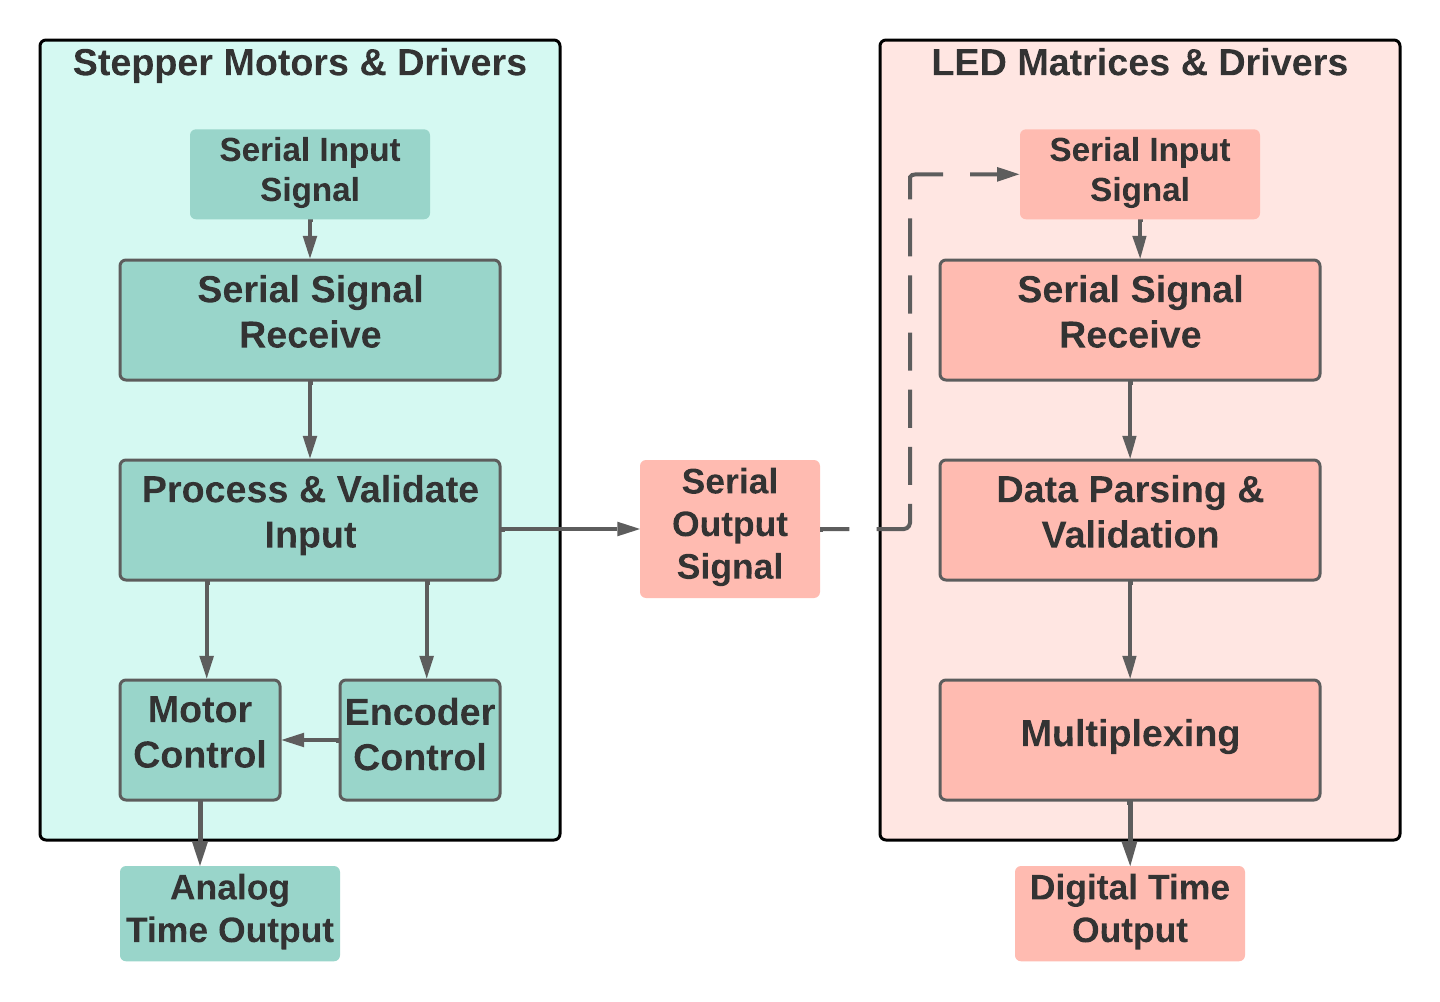
\includegraphics[width=4.4in]{LED_Motor_Block_diagram.png}
\caption{Software Block Diagram of Stepper Motor and LED Matrix Driver Serial Communications}
\label{SerialBlock}
\end{figure}

The ATmega board receives a formatted string through serial input from the \textbf{Flask} web framework and forwards it to the Tiva board before processing the input into the desired position of the clock hands. 
Similarly, the Tiva processes the serial input string, parsing it into which lights need to be turned on or off. 

This method allows for changes in both the digital and analog clock to happen simultaneously, while also allowing the \textbf{Python} aspect of the project to use a single serial port. 
Both microcontrollers individually parse and validate input into forms easiest for each display, and to ensure possible errors in input or corruption of input data does not impact the display at any stage. 

\section{Project Details}
\label{details}

Now that an overview of the project has been presented, a deeper explanation of the design process of the project will be explored. 
A detailed parts list can be found in Appendix \ref{appendix:parts}.
%set of schematics and a parts list can be found in Appendices \ref{appendix:schematics} and \ref{appendix:parts} respectively.

The details will be discussed in three primary sections. 
The first, Section \ref{MechDesign} discusses the mechanical and physical considerations, constraints, and design aspects of this project, and how they impacted other aspects of the project design. 
Section \ref{HWDesign} discusses the component selection and design process with a focus on the hardware while Section \ref{SWDesign} discusses the external software selection and design process with a focus on the project's software. 
Hardware and Software are further broken down into important blocks to be discussed in more depth. 

\subsection{Mechanical Considerations and Design}
\label{MechDesign}

The scoreboard central to this project provided several unique constraints with its history as an antique. 
Its exact age is not known, with an estimate of late 1950’s or early 1960’s from the client, and the company that had created it no longer exists. 
There was no user manual or specification document about the scoreboard, meaning information on its operation had to be uncovered empirically. 
%Nuri's feedback:
The scoreboard was constructed 
%without a way
with minimal regard to future internal access.
Additionally, there are indications that the scoreboard was built by hand, as several of the components show increased tolerances or imperfections.

%It quickly became clear in the process of taking the scoreboard apart that it was not constructed with access to its internals in mind, with only a few oddly sized and spaced holes in the device's face. 
%It also became obvious that it was likely built by hand, as several part of the chassis had imperfect cuts and uneven screw holes visible from a simple glance. 

%One of the primary instances where the mechanics of the scoreboard provided complications for the design process was in the analog clock. 
The analog clock of the scoreboard was originally designed as an 8-minute timer. 
Its construction complicated the design process because the clock hands were locked into an 8:1 ratio. 
This created the need for more discrete control of the clock hands. 
The choice to control the hour and minute hands individually was made because to provide any desired function that could mechanically facilitate, including future improvements.
%The part that became the analog clock face originally was used for an 8 minute timer for basketball periods. 
%The hands of the 8 minute timer, with one hand being minutes and the other seconds, were controlled through a single motor and single external hole in the clock face, as the hands were moved through concentric round shafts, allowing independent movement of both hands. 
%While it was originally believed that only the motor would need replacement, it was discovered when the scoreboard was opened that more changes would need to be made, as the existing gear box, corresponding to the 8 minute timer, had a gear ratio that meant that every full rotation of the minute hand would always correspond to a 45$^{\circ}$ movement of the hour hand when a 30$^{\circ}$ movement is what is necessary for a 12 hour clock. 
% A complete redesign of a gear box did not feel feasible for this project, as gears were not something either member of the design team had extensive experience in. 

Because the clock hands move independently of each other, and the installation would be wall-mounted, an open-loop control system (used in most analog clocks) would likely be too lossy to achieve the desired accurate timekeeping to the minute. 
To facilitate this, the clock hands needed to be tracked with feedback to the microcontroller driving the stepper motors.
A new gearbox was designed with regard to the constraints the chassis' small access holes and uneven cut-outs provided. 
Behind the clock face, the access hole for the plate for the motors was a mere 9.9 cm wide by 11.8 cm in length, with a depth of only 14.1 cm into the chassis. 
%When the decision was made to have a motor and rotary encoder for each clock hand, 
The shallow depth constrained all iterations of the gearbox design, as the team's choice to use one motor and rotary encoder per clock hand caused the gearbox depth to increase from its original size. 
The use of concentric shafts and pinion gears helped ease the restriction.
%became a problem that had to be solved with the usage of three metal re-purposed RC car pinion gears, as otherwise there was not enough depth for everything that needed to be connected to the concentric shafts. 
Relevant design choices will be discussed in greater depth in Section \ref{MotorDesign}.
The solution, the layout of which can be seen in Figure \ref{MotorLayout}, was the use of shaft couplings and the aforementioned gears to keep both encoders and motors within the necessary depth, but able to control the shafts independently. 
A custom shaft to fit the existing holes in the mounting plate, use the new pinion gear, and properly fit the smaller shaft inside with low friction was designed to meet these needs. 
% Put an image here of the new gearbox layout with a white background and do some explanation

\begin{figure}[H]
\centering
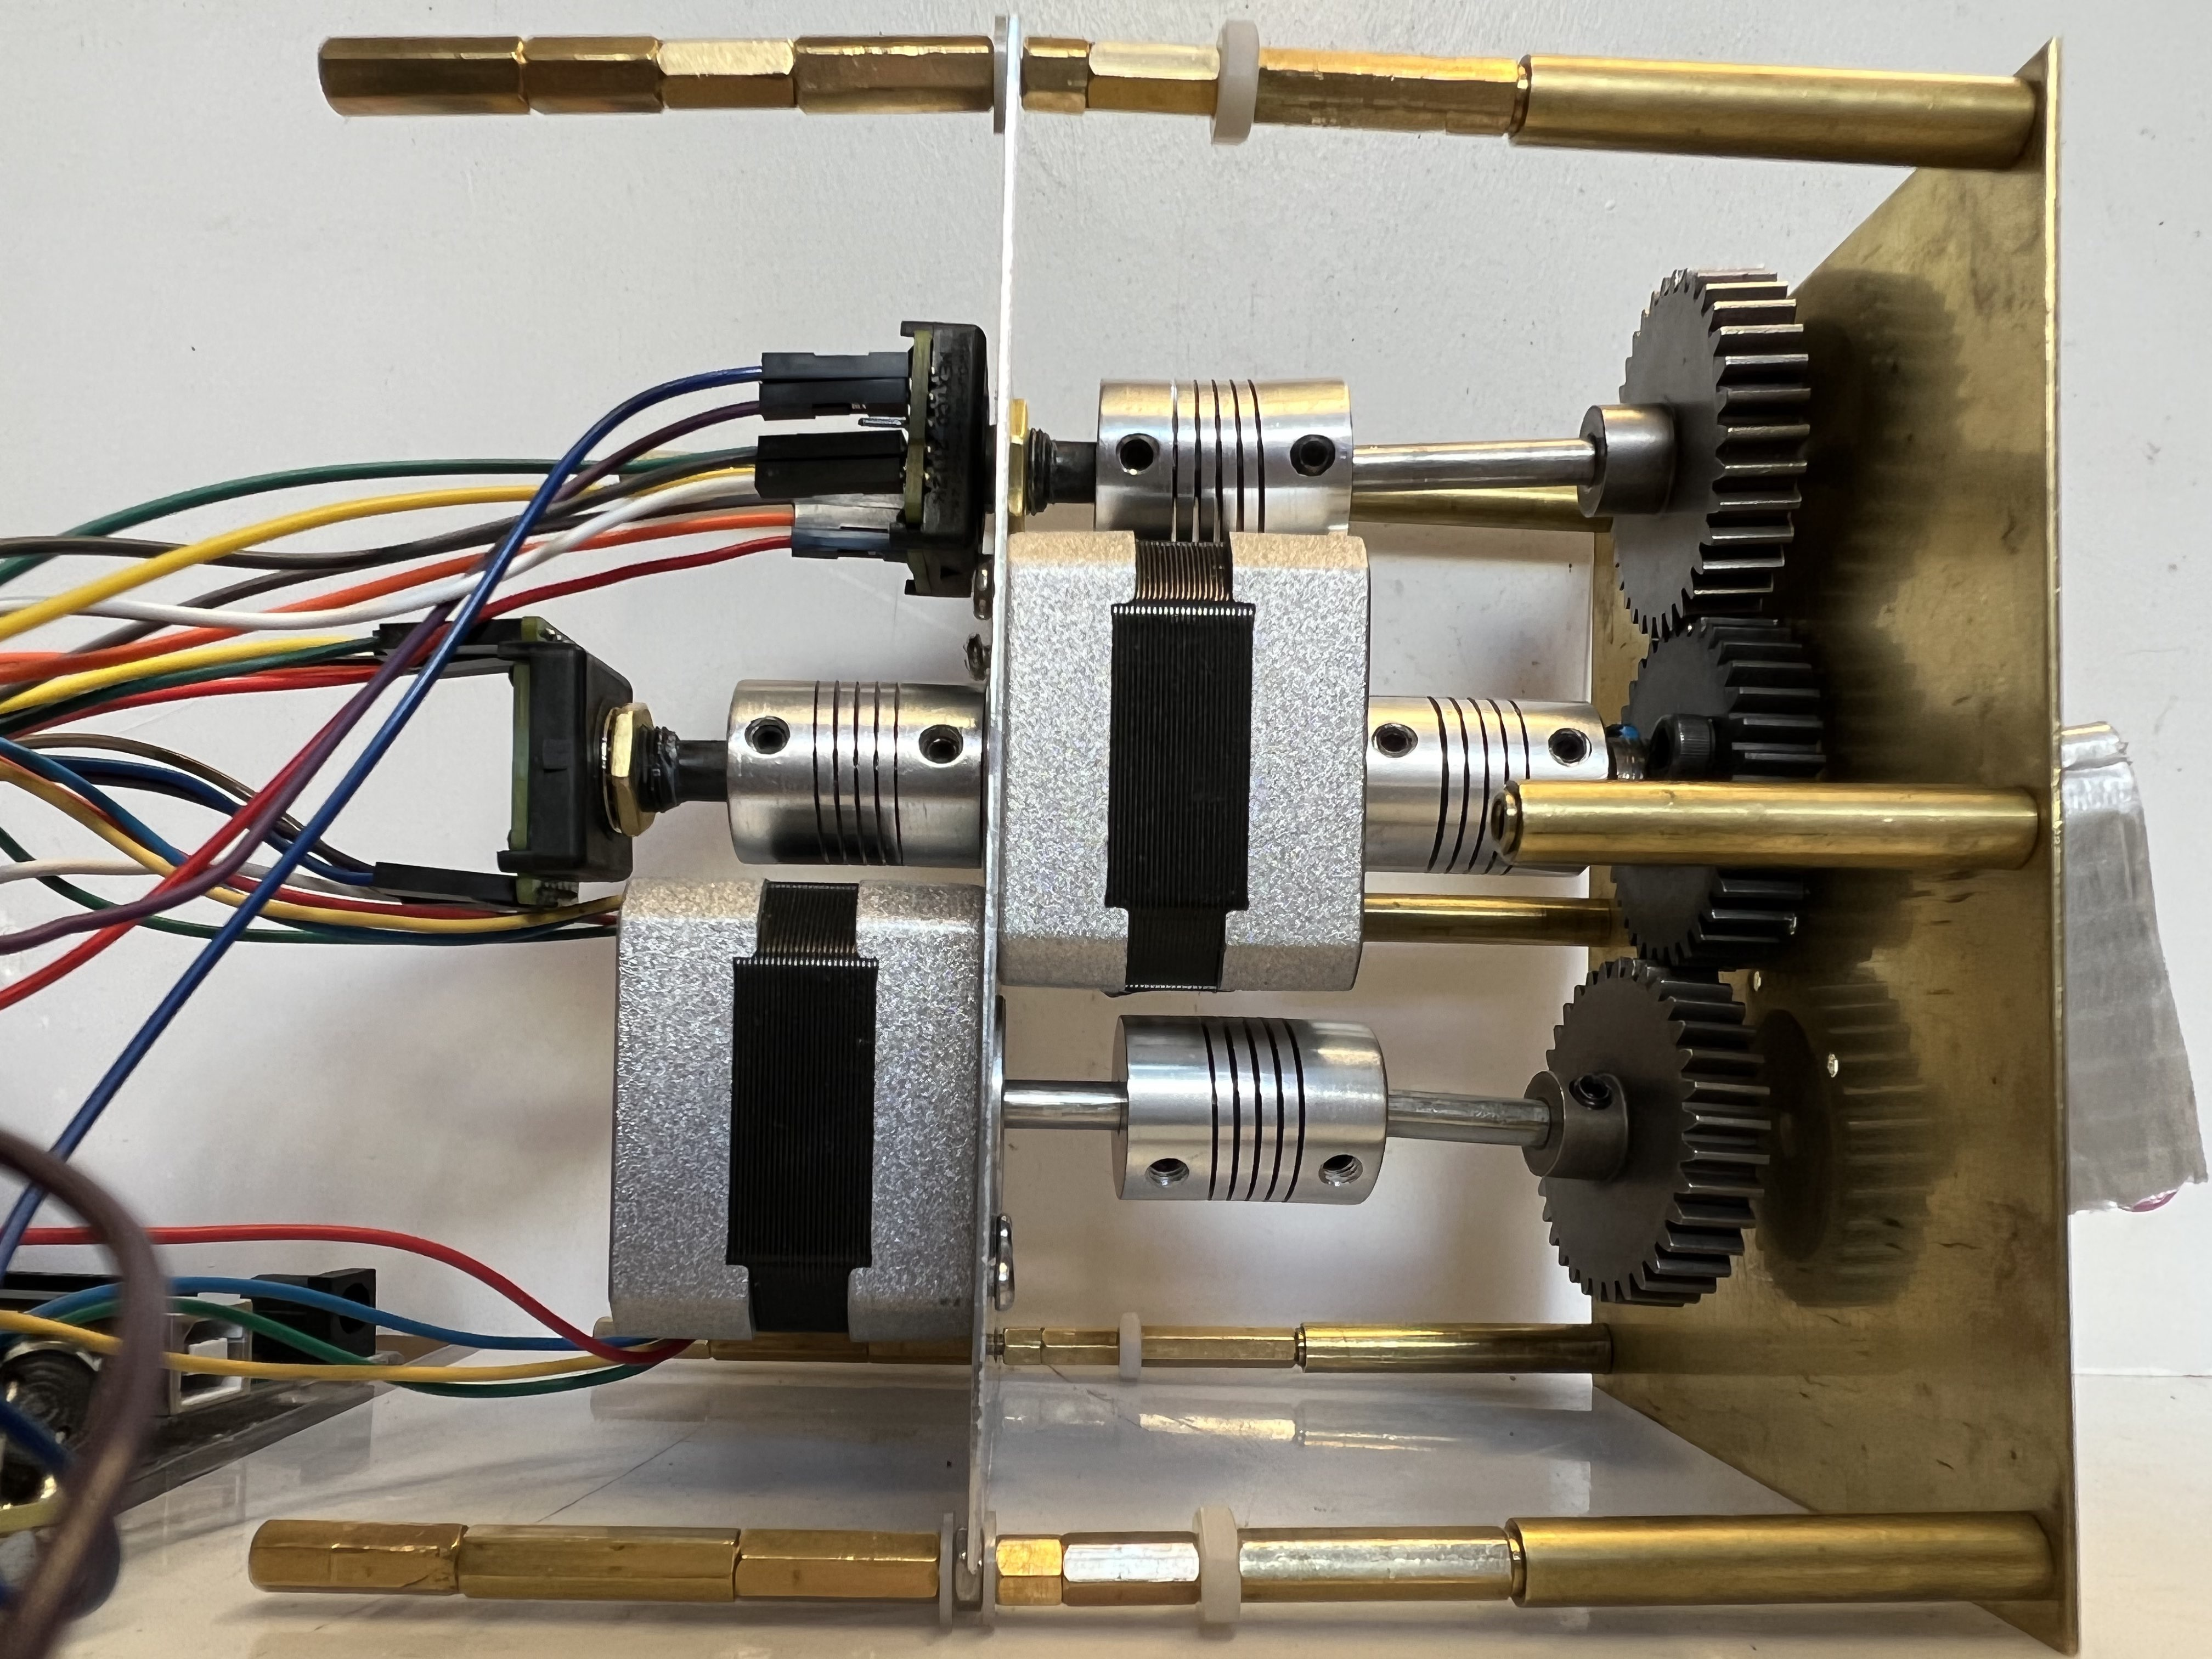
\includegraphics[width=4.5in]{motors.jpg}
\caption{Layout of Clock Hand Shafts, Motors, and Encoders}
\label{MotorLayout}
\end{figure}

The central shaft connects the minute hand stepper motor to a shaft coupled to the minute hand rotary encoder. 
The outer shaft for the hour hand has a pinion gear, which meshes with other identical gears.  
%each of which was then connected through shaft coupling to the hour hand stepper motor and rotary encoder. 
A gear train connects the hour hand stepper motor to its respective rotary encoder.

Other mechanical problems involved the need for custom metal plates for keeping the components stable, gear teeth together, and encoders steady, all intended to minimize error in time measurement.

% I really really didn't want to touch what you said here, but there was a grammar error that affected comprehension. --MM
%A mention that must be made is a massive thanks is owed to 
Massive thanks go out to Professor Joel C. Anderson of the Mechanical Engineering Technology department, and Stephen Abbadessa of the Mechanical Engineering department. 
Joel was instrumental in the design and manufacturing of the custom new shaft for the hour hand, as well as the structural plates necessary to keep the motors and encoders in the position they needed to be. 
Additionally, Stephen (or as he prefers, "Abbadessa") assisted by providing further mechanical engineering advice and services, namely machine shop training and additional structural plates for the gearbox.
%Both showed kindness and open-mindedness, as well generosity with their time and knowledge. They always tried to help bring out the best solution as the team presented design ideas.


% gearbox
%for the control of clock hands, had limited depth into the board, forcing creativity with the set up of the motors and encoders

\subsection{Hardware Design}
\label{HWDesign}

This section will provide a more in-depth look at the hardware of this project, including the justification of the selection of certain components, and the design of others. 
It is significant to note that at the time of this project's design and construction, global supply chain breakdowns hindered the team's ability to procure components.
%One thing of significant note in the discussion of selection of hardware and components is the time period in which this project was completed was during a global pandemic. 
The supply issues and shortages negatively impacted the availability of parts for selection, and required adapting and adjusting plans based on what was in stock. 
This was true for the selection of all components, but will just be stated here as not to be redundant. 

\subsubsection{Power Supplies}
\label{PowerDesign}
%% Overzealous power stuff begins
Power is provided to the device through its input, a NEMA 5-15 extension cord. 
To power the device, the NEMA 5-15P plug that extends from the device chassis plugs into a NEMA 5-15R receptacle supplying single-phase 120 $V_{rms}$. 
Power supplied at 120 $V_{rms}$ using either NEMA 5-15 or NEMA 1-15 plugs, receptacles, or sockets will be herein referred to as "mains power".

% The power input of the device referenced as the input of a wall outlet refers to the US household standard of 120 $V_{rms}$. 
Using a grounded extension cord (NEMA 5-15), the device is connected to mains power. 
Internally, the socketed end of the extension cord mates with a plug, extending mains power to 3 NEMA 5-15R sockets for use in AC-DC power supplies. 
The Raspberry Pi is supplied 5.1 VDC at up to 3 A by a Raspberry Pi 15W Power Supply (the official and recommended PSU), which is itself supplied power at 120 $V_{rms}$ from an internal NEMA 5-15R socket.
% talk about how meanwell was chosen after the selection of motors so we knew 12V was needed

Additionally, a Mean Well RS-15-12 unit, capable of supplying 12 VDC at up to 1.3 A (totaling 15W), is supplied power at 120 $V_{rms}$ from another internal NEMA 5-15R socket. 
The stepper motors used to drive the analog clock and the LED multiplexer PCB used to drive the digital clock require 12V DC to run.
Previously, a 4th outlet terminated the aforementioned internal strip of mains power outlets. 
With the addition of the Mean Well power supply unit, a device powered through its screw-terminal connectors, the 4th socket was cut off the internal mains power strip to meet this need. 
The power strip is now terminated using the Mean Well PSU, by tapping the wires that ran to the old 4th socket.
% serves to provide the necessary 5 VDC power for the Raspberry Pi through a standard wall mount adapter, as well as to then connect to a 12 V, 15 W Switching Power Supply to provide the necessary 12 VDC for the stepper motors and the LED Multiplexer PCBs. 

The ATmega and Tiva boards also require power at 5 VDC, and less than 2.5W each, which can be provided by the Raspberry Pi. 
The power is supplied to the microcontrollers using USB-A plugs and sockets in compliance with the USB 2.0 standard's power specifications. 
The stepper motor drivers used also required 5 VDC, which was provided through a connection to the ATmega board. 
%% Overzealous power stuff ends

\subsubsection{Motor \& Motor Driver Selection}
\label{MotorDesign}
% 1 motor vs two, full gear box or not
% making one dual shafted 
% stepper motor because of holding torque vs dc or servo, low speed and high precision
% servo mostly only 180 deg max

% I think this might all be too much detail, idk, its weird 

% motor selection
When deciding on which motor to use for the control of the clock hands, two decisions had to be made.
The first was the quantity of motors used (one for both motors or one for each motor), and the second was the type of motor(s) to use. 

%The choice of one motor or two was influenced greatly by the mechanical constraint of the  realization that the original gearbox would not work for our purposes after significant time spent attempting to have it function as desired. 
The original design had one motor connected to a gearbox with an 8:1 ratio between clock hands, but that would not function for the 12:1 ratio needed for a 12-hour clock.
This provided two options: a single motor and a new custom-made gearbox to ensure the proper ratio or a pair of motors with each clock hand having its own independent motor. 
Both a lack of background in the design and manufacturing of gearboxes, and the potential benefits of having independently controlled hands, led to the decision to have two separate stepper motors.

% discuss types of motors, dc vs servo vs stepper
Another key decision to be made was the type of motor to be used. 
The three primary types are DC motors, stepper motors, and servo motors.  
While each has its own advantages and disadvantages, DC motors function best in applications with a high RPM value and Servo motors are most often found with a maximum of 180$^{\circ}$ of rotation. 
For an application where there would be most often $1/60$ and $1/720$ RPM, DC motors would not be practical, and 360$^{\circ}$ motion being necessary for clock hand motion meant that servo motors similarly would not be a reasonable solution. 
Stepper motors are the optimal choice for slow and precise motion, and provide high holding torque. 
%Especially for the hour hand, and in comparison to the available speeds of the stepper motor, the hands would be very slow moving. 
The clock hands will rotate very slowly ($1/60$ RPM and $1/720$ RPM) so stepper motors were chosen.
200 steps per rotation is standard for hybrid stepper motors. 
%With 12 hours on the face, each hour would be represented by just under 17 steps, leading to a delay on the order of minutes between each step. 
Additionally, stepper motors can provide the holding torque necessary to keep the clock hand in position without overheating.
Tracking of the hands' angular positions is further discussed in Section \ref{PositionDesign}. 
Stepper motors also come in the form of bipolar or unipolar, based on the polarity of the internal solenoid coil and the capability to handle current flow in one or both directions. 
Bipolar motors are typically more efficient and have higher torque, though they typically require more complexity to control and drive. 
That is why stepper motor driver boards were used.

%maybe add in actual equations here ^? Make this have specific numbers so it looks official and everything, esp. since you don't have a lot of actual equations elsewhere

%motor driver selection
The original motor driver board intended for use was the TMC2208-LA SilentStepStick stepper motor controller and driver. 
Noise, in terms of vibration or sound, could be particularly noticeable in this application, with most components of the analog clock being made of metal and therefore causing resonance and creating noise. 
Trinamic Motion Control (TMC) motor drivers are known for particularly quiet motion.
Notably, 3D printing communities use Trinamic stepper motor drivers to reduce motion noise by 100x, as compared to less-sophisticated but common stepper motor drivers.
The TMC220X \& TMC213X series drivers are commonly used, so many resources already exist for their support, including Arduino libraries. 
With the aforementioned shortages, one of the only TMC220X or TMC213X series drivers available was the TMC2209-LA SilentStepStick, and as such was the one selected for use. 
The SilentStepStick series has microstepping and a capability known as stealthChop, both of which provide quieter operation. Microstepping allowed for more effective resolution of steps per rotation without having to purchase a more expensive stepper motor.  


% Trinamic driver wanted, known to be quiet, people in 3D printing use them for 3D printers that operated silently, its why we wanted TMC220X & TMC213X series. Drivers other than the 220-9x were mostly out of stock, so the 2209 driver was chosen in the interest of sustained obtainability.

%The TMC2209 had a property known as stallGuard, said to provide the capability for sensorless motor load detection, % add citation in here 
%which was originally thought to be able to provide the desired position tracking of the clock hands throughout their rotation, but further investigation found stallGuard to be best applied in applications of linear movement with clear bounds, not continuous rotational movement. 

\subsubsection{Rotary Encoder Selection}
\label{PositionDesign}
% Hall sensor attempt, considered holes in the board and light sensing used, before settling on rotary encoder and the complications involved, original concern with the encoders was the ability to have it remain accurate even if hands are moved when it is off, which is why HW zero was used, decided after to also provide a software zero in case of encoder not remaining consistent 

To meet the project specification of accuracy to the minute for the analog clock, a method had to be found to determine where the hands are at any given moment so their position could be properly adjusted accordingly if needed.
% Unlike servo motors, stepper motors do not have set programmed positions, and it was too late into the project that it was discovered that there are some stepper motors available with built in encoders to solve that issue. 
% Instead, a method of keeping track of the position of the hands had to be selected. 

% Two methods were considered but not selected for the final design. 
% The first of such methods was the usage of a Hall effect sensor. 
% A Hall Effect Sensor senses the change in voltage due to the movement of a magnetic field, with a signal strength corresponding to the magnitude of that field. 
% Hall sensors are commonly used in industry for applications of speed of rotation, or as a magnet controlled switch.  

% The plan had been to have Hall Sensors set up in locations that would allow for homing the hands at a set time. 
% One sensor would be placed where the tip of the minute hand would pass over it, and the other placed where the tip of the hour hand would pass over it. 
% This idea experienced several problems in execution that made it not a feasible solution. 
% With the spacing between the hands, the hour hand was raised near 0.5 cm off of the clock face, while the minute hand was raised near 1 cm off of the clock face. 
% The clock face, scoreboard chassis, and clock hands are all made of ferromagnetic metals, and none of the three were parts that the client wanted to replace. 
% For a magnet to be strong enough for the hall sensor on the clock face to detect its movement, it was often strong enough to cause the clock hand to get stuck to the clock face. 
% Besides slowing the movement and causing inaccuracy in time, this would scrape the paint of the clock face over time, and also lead to the clock hands getting stuck together which is significantly more problematic. 
% With many similar applications making use of the Hall Sensor, it had seemed ideal, but in actuality was not practical for this project. 
% Another solution had to be found. 

% Another method considered had been the usage of light detection sensors. 
% A pair of small holes would be drilled into the clock face and chassis, and light detection sensors would be installed in those holes, such that when both detect darkness, that means that one hand is over each of them. 
% A lack of knowledge on the lighting situation of where the scoreboard was to be installed and the sheer variety in potential lighting provided too many unknowns for reliable design, so other options were considered. 

A solution was found to be the use of a rotary encoder.
Specifically, a mechanical continuous absolute contacting encoder (ACE) with 128 absolute states was used. 
A rotary encoder utilizes various methods, in this case mechanical means, to convert the angle of its shaft into a digital output signal. 

Continuous indicates the ability to detection full rotations of the encoder, and that a limit will not be reached after a certain amount of degrees of rotation. 
An absolute rotary encoder outputs based on the absolute position or angle of the shaft, which can be maintained even when the device is turned on after a period of being off. 
An incremental encoder, in comparison, has its output based in the motion and change of angle or position. 
For this application, for keeping track of the position of the clock hands even if the hands were moved while it was off, an absolute encoder is then the best choice. 

An encoder with 128 absolute states was used to ensure that, for the 360$^{\circ}$ of rotation, every minute would have at least 2 states of the encoder. 
An additional advantage to the specific encoder used, a Bourns EAW ACE-128, was the existence of a reliable MIT license Arduino library. 
This meant that the position to binary mapping of the 128 separate states, where the decimal output was not directly sequential with the position value, did not have to be done by hand. 
With separate non-sequential 8-bit binary output codes for each of the 128 positions, this not only saved significant time, it also decreased the chance of error from misplacement of any of the 1024 bits that had to be mapped. 

%Talk about what each of those keywords mean and why we want them for this project, 128 states to try to ensure accuracy to the minute, at least 2 states for each minute, an arduino compatiable library for this encoder was found to ensure smooth use without having to hand program translation of the binary output, KEYWORDS: Mechanical, Continuous, Absolute

\subsubsection{Microcontroller Selection}
\label{MicrocontrollerDesign}
% Talk here about how an Arduino Uno was originally used, until, with both encoders and motors, ran out of serial inputs. Uno with Nano was attempted, until the decison was made to use the ATmega board, an Arduino Mega clone used because of supply chain complications

% In early stages of design, for the motor control, an Arduino Uno had been used. 
% It had a single hardware serial port, 11 available Digital I/O pins, and 7 available Analog I/O pins that could be re-purposed to be Digital I/O. 
% Pin 0 and 1 of the Arduino Uno are the RX0 and TX0 pins respectively, and are not available to be used as Digital I/O when the serial port is in use. 
% This leaves effectively 18 pins available for the motor driver board and rotary encoder pins, which was not enough. 
When selecting the MCU that would be used for the control of the Analog clock, I/O and Serial communication were two of the primary factors examined. 
Each rotary encoder required 8 Digital I/O pins and a connection to ground. 
Each motor driver required 5 Digital I/O pins (with two of those requiring Pulse-Width Modulation (PWM) capability) as well as a connection to ground and a connection to 5V. 
With two encoders and two motor drivers, that is a requirement of 26 Digital I/O Pins to connect the hardware of the clock to the MCU. 
An Arduino Mega has 54 available Digital I/O pins, with 15 of them capable of PWM. 
It also has 3 serial ports which were used to provide a serial connection to the Raspberry Pi as input and to the Tiva board as output. 

However, with a lack of available stock and delay in shipping from the aforementioned supply chain issues, a clone of the Arduino Mega, the ELEGOO Mega R3 ATmega board, was instead used. 
%% need to add transitions here between different microcontrollers
%Talk here about the Tiva

Where the ELEGOO ATmega board runs the mechanisms of the analog clock, its counterpart which runs the digital clock display is a Texas Instruments Tiva C-Series microcontroller. 
This was selected to drive the multiplexed digital clock display. 
Its purpose, more specifically, is to toggle the gates of NMOS transistors on the multiplexing PCB, ultimately controlling the on/off states of the LED matrices and their respective pixels. 
The microprocessor at the core of its design is the TM4C123GH6PM, capable of 100 Dhrystone Millions-of-Instructions Per Second (DMIPS) of performance when running at 80 MHz. 

\subsubsection{LED Matrix Control PCB Design}
\label{PCBDesign}

%Miles will talk about PCB stuff here.

% VERY ROUGH DRAFT. DO NOT FEAR THE BRAIN DUMP.

Initially, the project was not obligated by its contract to create and utilize a printed circuit board (PCB). 
However, in the interest of continued function, replaceability, and ease of repair, a PCB has been designed and manufactured. 
Prior to the circuit board's manufacture, a breadboarded circuit was used, which went through several revisions. 

\begin{figure}[H]
\centering
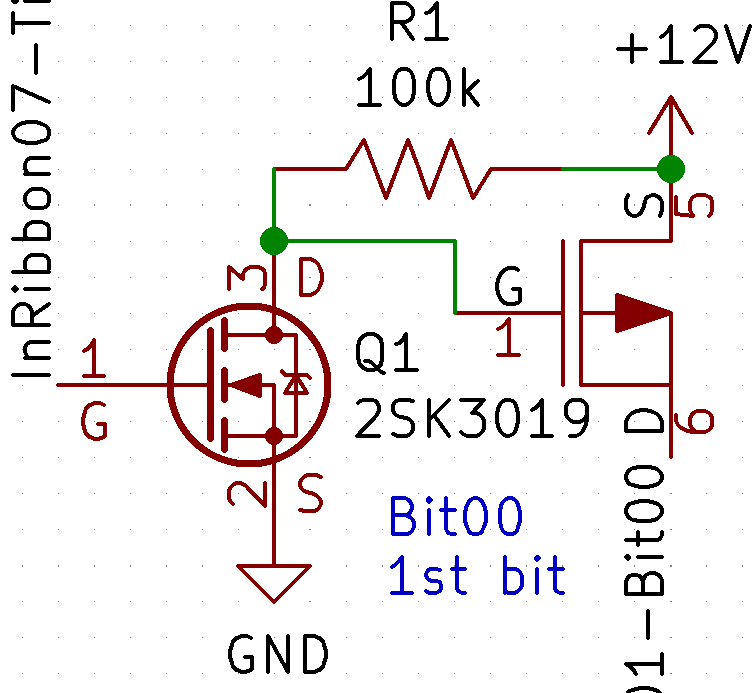
\includegraphics[width=2.5in]{basic_transistor_circuit.png}
\caption{The pullup circuit used, consisting of a PMOS transistor (right) driven by an NMOS transistor (left).}
\label{transistor_pullup}
\end{figure}

The unit seen in Figure \ref{transistor_pullup} is the pull-up circuit, which allows the high-voltages to electrically connect to LEDs which should be illuminated. 
There are 22 of these, one for each electrical connection to a bulb or set of bulbs in the digital clock display per matrix. 
Inbetween the drain of the transistor at the right (Fig. \ref{transistor_pullup} and the anode of the diode in Figure \ref{transistor_pulldown}, the pulldown circuit, would be between 1 and 4 LEDs, due to four copies of the circuit in \ref{transistor_pulldown} being present on the circuit board. 
\pagebreak

4 LEDs is possible if the grounds are not being multiplexed, but under normal multiplexed operation, only one LED bulb will be electrically connected to these points in the circuit at one time.

\begin{figure}[H]
\centering
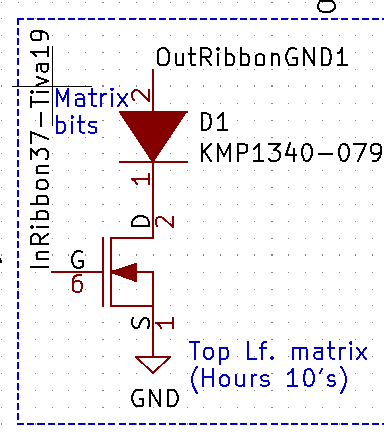
\includegraphics[width=2.5in]{basic_transistor_unit_down.png}
\caption{The pulldown circuit used, consisting of a diode (top) feeding into the drain of the NMOS transistor (bottom).}
\label{transistor_pulldown}
\end{figure}

% Initially, this arrangement was prototyped in a 1-by-1 fashion, where multiplexing routines could be tested to some extent. 
% This was eventually extended to a 1-by-8 array, representing the 8 lights across two matrices. 
% This array 
% A circuit was built with 8 multiplexed ground connections and 15 multiplexed +12V connections so that all the lights on the display could be multiplexed. 
% However, due to a common-cathode configuration, this idea was not used, and so a circuit capable of driving 22 LEDs with 4 separate grounds was designed instead. 

This arrangement was prototyped in a 1-by-1 fashion, where multiplexing routines could be tested to some extent. 
A circuit capable of driving 22 LEDs with 4 separate grounds was designed instead. 


The PCB was constructed in KiCad and was assembled by JLCPCB using pick-and-place assembly for the surface-mount technology (SMT) as well as hand-soldering for through-hole components. 
The design features two sets of pin headers for data/signals and a third set of pin headers for power to the board, all which were hand-soldered. All other materials in the "PCB Components" section of Appendix \ref{appendix:parts} were soldered with pick-and-place machines prior to shipment. Future iterations may come with all parts soldered to simplify the client-side labor and repair process, should the need arise. 

%First, breadboarded after conferring with professor. Then
%with breadboard circuit implemented, 1x1 multiplexing was achieved. a 8x15 (7.5x4x4) array was initially selected, designed, and eventually assembled, but then it was realized that the scoreboard chassis functioned as a common cathode. This forced the display to have dimensions of 1x22x4, and the transistor logic polarity had to be inverted. Initially the polarity didn't matter because the LED bulbs chosen have built-in rectification circuits (in addition to current limiting). Another contrast between the two designs is that the entire matrix panels would be multiplexed, not just single rows as was initially envisioned. Additionally, the pins of the wiring harness did not have a 1:1 mapping with the lights of the LED matrices  

%To keep costs low, many parts were salvaged or obtained at no additional cost. Two IDE-style cables were salvaged, and the Tiva C board was obtained at no additional cost. Other prototyping materials such as breadboards, wires, and components were obtained at no additional cost from the Whitney Lab parts cabinet. 




\subsection{Software Design}
\label{SWDesign}

The various software components that control the various aspects of the scoreboard are described in the following section. 
First, in Section \ref{FlaskDesign} will be the discussion of the \textbf{Python}-based \textbf{Flask} Web Framework, with its associated GUI and the development of the UI. 
Section \ref{SecurityDesign} details the security measures added to the Pi's OS. 
Then, Section \ref{AnalogDesign} discusses the software controlling the analog clock while Section \ref{DigitalDesign} talks about the software controlling the digital clock. 
It will be concluded in Section \ref{RTCDesign} with discussion about the methods considered and the one selected to maintain accuracy of time for the project. 

\subsubsection{Python-based Flask Web Framework}
\label{FlaskDesign}

The web framework, as well as the User Interface (UI), for this project was accomplished through \textbf{Python} with the usage of the web framework \textbf{Flask}. \textbf{Flask} was built to support extensions and APIs to add in whatever functionality a user needs for individual applications.  One example used in this project would be Turbo-Flask, which was used to keep a live display of the current system time of the RPi on the GUI.


% The UI was one of the first aspects of software developed for this project, as it was something that neither of those working on this project had extensive prior experience with. It served as something productive to work on while key parts were in the process of being shipped and delivered.
% While this initially seemed to be the ideal method, it came with a few problems. 

% Originally, the interface was rather extensive, made purely of HTML supplemented with Javascript and CSS, and even contained the start of a live model of the scoreboard complete with a functioning clock. 
% Particularly from someone with no prior HTML experience, the development of that UI was a significant time sink, particularly as it did not make it to the final GUI. 
% That being said, the learning experience of that those hours spent did make the later design of the html page template for the \textbf{Flask} framework much easier. 
% One of the mock-ups of the HTML/CSS/js prototype GUI can be seen in Figure \ref{protoGUI}.

% \begin{figure}[H]
% \centering
% 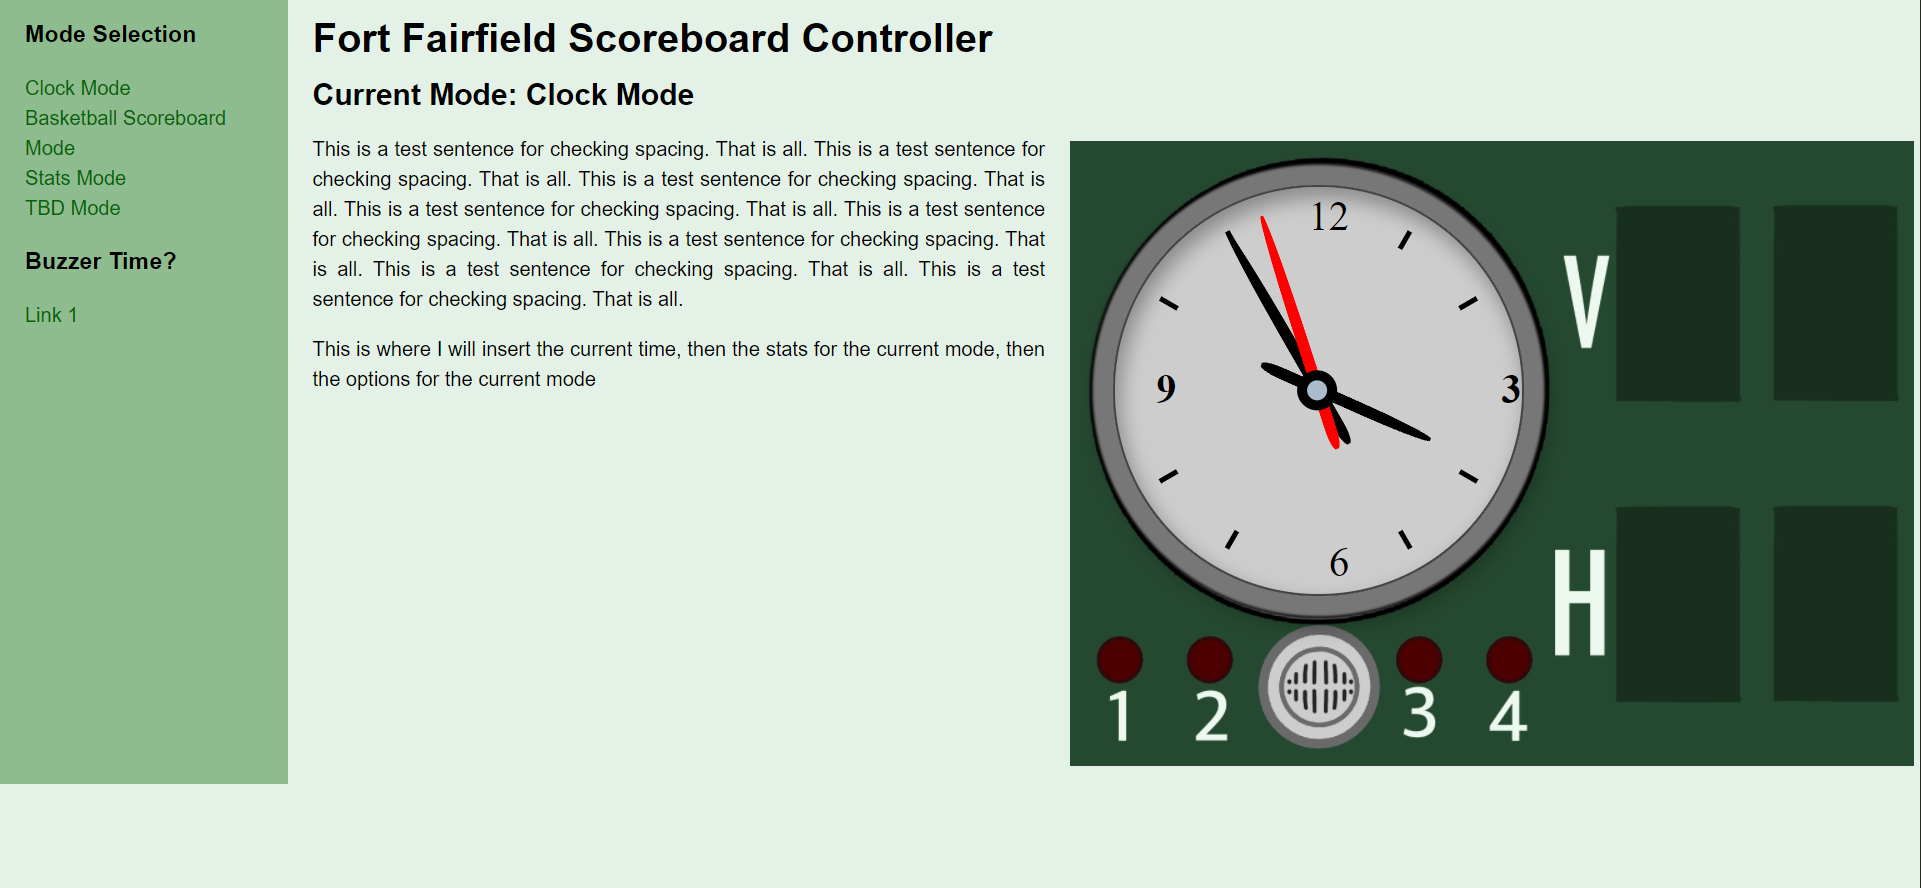
\includegraphics[width=6.8in]{htmlProto.png}
% \caption{HTML managed Prototype Graphical User Interface (GUI)}
% \label{protoGUI}
% \end{figure}

% As was discovered through the implementation of switching between modes of the scoreboard (a functionality that was considered in early stages of development), communication between separate HTML pages is not easy to achieve, and duplex communication between HTML and other file types, such as serial connection to the control code as would be needed, is even more difficult to achieve without a more well-rounded programming language than HTML on its own. 
% For that reason, other methods for creating the web-based GUI were investigated. 

% The solution that was then settled upon was \textbf{Flask}, a \textbf{Python} based web framework to create the desired web interface with ease, simplicity, and functionality. 
% \textbf{Flask} itself, when used in this application, is able to call HTML files as something called template files. The GUI itself could be created in HTML, but the functional back-end of the web server would be in \textbf{Python}, providing much more reliable and clearer functionality. 


For this project, the "\textbf{Render Template}" \textbf{Flask} method was used to load the GUI that was written in HTML and allow for the exchanging of data between the GUI and \textbf{Python} script. The GUI itself could be created in HTML, but the functional back-end of the web server would be in \textbf{Python}, providing much more reliable and clearer functionality. The "Request" method was used for receiving user input from the GUI through HTML forms. 

The \textbf{Python} script begins by connecting to the ATmega board through USB Serial, and then defines the input collection, starts the thread for updating the system time display without a page refresh, and configures the serial output of the GUI before actually starting the GUI. 

User input being received and then used to control the clock can be seen after the user selects a button or a time to display, as that data is then sent from the \textbf{Python} script to the other control scripts, which have a clear visual change (such as movement of clock hands). 

With this method of communication, an extra layer of security is created, as the user input can only be in the form of whether a button is pressed or not, or in the form of HTML input type time, which contains its own data validation that ensures that input will always be in an expected form. 
This is important, as the board will be in a public location. While there are security measured ensured (as will be discussed in Section \ref{SecurityDesign}), even if an unintended user gains access to the web page, the available inputs are all limited. It would all control input that could be easily with selecting a the GUI option to reset to current system time. 

Figure \ref{UI_trace} provides the path of data from user input (as a button press or HTML time object) to serial output to the Analog Clock MCU. The examples of possible input and the corresponding output the MCU would receive use an arbitrary current system time of 9:24am. 


\begin{figure}[H]
\centering
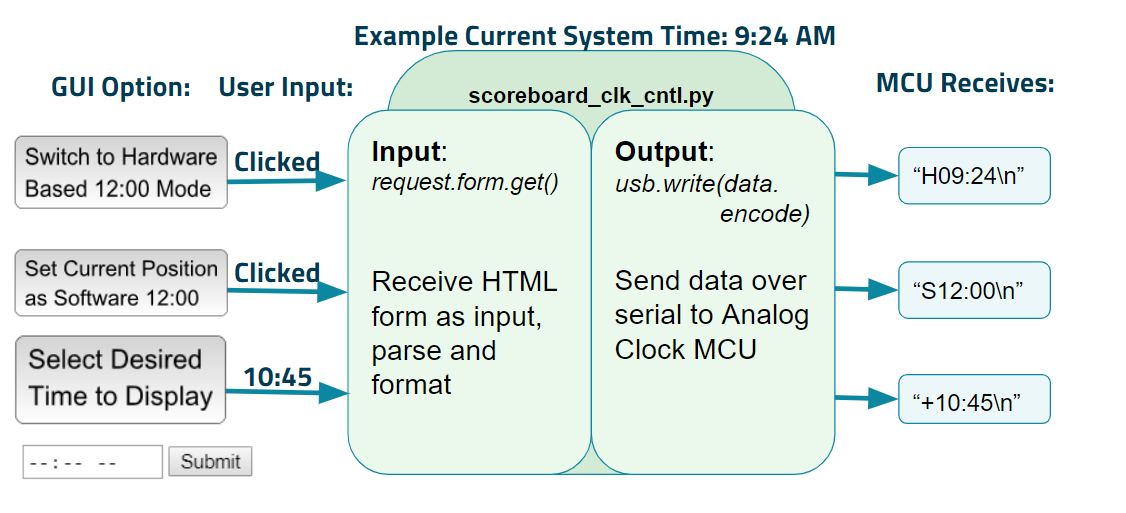
\includegraphics[width=6.8in]{tracingGUIInput.PNG}
\caption{Tracing User Input from Graphical User Interface (GUI) to the Analog Clock MCU}
\label{UI_trace}
\end{figure}

The user input received is parsed and then must be arranged in the desired format for the analog clock MCU. That format, with HR representing the two digit hour (zero-padded as necessary) and MN representing the two digit minute (also zero-padded as necessary). 
The string format sent would be "+HR:MN\textbackslash{n}", with + representing the intended function for the control code scripts to receive, and then the two digit hour, a colon, the two digit minute, and then a newline. The symbol, indicating the unique function, before the time is a specific capital letter (U,H,S,R,D, or M) or the '+' symbol. Only strings that begin with one of those symbols and then has the proper formatting of the time are actually able to change the visual clock display. 
Once formatted, the is data then encoded and written to the USB serial connection for the Stepper Motor MCU to receive as serial input.


% Mention how, with the way user input is captured,parsed, and sent, with multiple layers of parsing and validation, even if someone managed to access the webpage, the worst they could do is make the clock display an inaccurate time, 

\subsubsection{Operating System Security Measures}
\label{SecurityDesign}

%Create new user with unique username and password
%Disable pi user
%Change the SSH port
%Change the VNC port
%Use key-based SSH access only
%Disable and remove mDNS advertisement/services
%Disable ping responses
%Install and configure firewall (ufw)
%VNC only accessible when forwarded through the SSH tunnel

To facilitate \textbf{Flask}'s services, it was necessary to network the RPi. 
The RPi was connected to the internet using the University of Maine's "tempest" Wi-Fi network. 
Making the decision to connect the Pi to the internet was deemed required for several reasons. 
Primarily, an internet connection to the RPi would facilitate the ability to develop code and test features remotely during the project's development phase. 
It was also necessary to install new programs (e.g. \textbf{Flask}), as well as update installed packages and programs aboard the RPi to their most recent versions.
This is considered necessary for Internet-connected devices within the domain of cybersecurity, insofar that devices should do so regularly while the device is connected to the Internet. 
In the time between the installation of Raspberry Pi OS and the connection of the RPi to "tempest", security researchers had uncovered severe vulnerabilities within standard packages (e.g. ssh-agent: CVE-2021-28041, March 2021) included with some modern Linux distributions.
Raspberry Pi OS was among these, at that time.
To mitigate potential cybersecurity threats and attack surfaces, many steps were taken to provide more advanced security measures to the RPi.
The most notable 9 measures taken will be discussed in the paragraphs which follow.

The first step taken upon booting the device was creating a new user with a unique username and password. 
The username "nema" was chosen. 
It is longer than the default username, "pi", so it is less easily brute-forced. 
A password was randomly generated using a password scheme. 
Subsequently, the "nema" user was given administrative privileges equivalent to that of the "pi" user, the "pi" user was locked to prevent further access, and the "pi" user's password was changed using the same scheme for randomly generating passwords.
Locking default users and changing the passwords from default values improves the security of the device because a malicious actor would not be able to rely on having credentials to the device, if networked or physical access is achieved.

To provide further security, the port for the Secure Shell (SSH) service was changed from the default (22) to a new, higher value (55155). 
The SSH service uses the Transmission Control Protocol (TCP) to transmit and receive data, so SSH uses TCP port 55155. %redundant but need to mention tcp somehow. TODO
This provides security because port-scanners and service enumerators rely on a combination of the port number, responses to enumerating queries, and other factors to assess what program is listening on that port. 
Now that the SSH server listens on port 55155, there is a decreased likelihood that a) the port will be scanned (lower ports are more commonly scanned) and b) the enumeration of the service would successfully identify the service listening. 
The SSH service is also configured to provide access exclusively to users who authenticate with a valid SSH key, keys which are designed to be virtually impossible to brute force.

Similarly to the SSH service, the Virtual Network Computing (VNC) service also had its port changed.
The VNC service is, in many default configurations, considerably more insecure than SSH, so in addition to changing the service's port from 5900 (TCP) to 51511 (TCP), a firewall for incoming traffic restricts access to all ports except 55155 and port 80. 
The presence of the firewall (run with "ufw", the "Uncomplicated FireWall") gives leeway for the VNC server to run in a more compatible configuration. 

The firewall configuration intentionally prevents ordinary users from directly connecting to the VNC server. 
This is because, in this project, the GUI remains installed for ease of administrative access. Forcing indirect access to the GUI increases security and accessibility at the cost of network connection latency. 
The latency is of minimal consequence if the administrator is experienced in using a Debian-Linux-based command-line interface (CLI). 
The limited speed of data encryption adds a significant amount of latency. 
Because CLI access over SSH requires the encryption of less data per unit time (as compared to VNC via SSH), CLI interactions are less affected by delay due to encryption times (latency).

Finally, services such as multicast domain name system (mDNS) advertisers (here, "cups-browsed" and "avahi-daemon") and "ping", a service used to enumerate hosts, were taken offline. 
Specifically, the "cups-browsed", "avahi-daemon", and "ping" services were all configured to respond to queries or advertise once their services started running at boot-time. 
The network traffic these programs are designed to produce would decrease give away the device's presence on the network, which is undesirable in this application.
"cups-browsed" and "avahi-daemon" are daemons, which are Linux system services that are meant to run unattended and, for the most part, uninterrupted. The change to the "ping" service required a change in kernel parameters, and the other two daemons were disabled and prevented from ever restarting using "systemctl", a daemon itself that manages other daemons. 

\subsubsection{Clock Hand Control}
\label{AnalogDesign}

% The minute and hour have different variables to ensure the moving to a specific time functionality only occurs after a proper serial input was received, with the value of minutes being 61 and the value of hours being 0, as 0 minutes should be a valid input. 


The software controls for the motor analog clock hand control was programmed  through an ATmega based clone of the Arduino Mega, programmed primary through the Arduino IDE. 

This facilitated the usage of libraries for both the TMC Stepper Motors and the ACE128 encoder. As previously discussed, bipolar motors have significant advantages over unipolar stepper motors, but are more complex to control, and the encoder used was ideal for the application but would have required significant and complicated bit mapping. 

While the encoders with the libraries could provide the rotary position, algorithms still had
In particular, functions were used for the conversion between the 128 encoder positions and 12 and 60 positions necessary for the hour and minute hands. There was a function for encoder position to clock hand position and vice versa for both minutes and hours, as the ratios were slightly different. Notably, 128 does not divide evenly by 12 or, by extension, 60, so this conversion algorithm would not be able to be perfectly evenly spaced. For the hour hand algorithms in particular, to compensate for this, the 8 remaining positions from evenly dividing by 12 were split among the hours on the top half of the clock. Hours 4-8 only consisted of 10 positions from the encoder, while the other hours consisted of 11. While the stepper motor selected has plenty of holding torque to prevent any slippage of the hand motion, it was thought that having the extra positions be in the top half could help compensate for the hand being suspended with its weight more against gravity.

To determine the mapping of the minute encoder value to hand position, actual calculation was done instead of hand-selecting values. An algorithm was made to ensure, of the 128 rotary positions, each minute has at least 2 unique positions. This was done by multiplying the raw position (an integer from 0-127) by the float 60.0/128.0 to represent 60 minutes spread over the 128 unique positions. Then, to get the integer representation of the current minute, that value is floored.This process ensures every minute on the clock hand was represneted by at least 2 encoder states to meet the specification of accuracy to the minute. 

    % //128 positions, so each minute is 2 2/15 (2.1333) positions
    % minFloat = rawPosition * 60.0 / 128;

% Stages, since it was lots of hardware working together, done in steps and then put together
% Stepper motor control
% Encoder reading
% stepper motor controlled by encoder
% two stepper motors each controlled by encoder
% receiving serial input from the \textbf{Python}

% The code was designed in stages, as it consisted largely of multiple pieces of hardware control working together. It was advantageous to get each piece of hardware working, and gradually combine them. First was the development of control of a single stepper motor, then the development of code reading from a single encoder. After both were in a functional state, code was developed for the control of a stepper motor by the input from a single encoder, and after that was functional, code was developed for having simultaneous control of two separate motors by two separate encoders from the same board. Finally, receiving serial input from the \textbf{Python} script was added, and the control algorithms adjusted to have both the serial input and encoder input used to control the stepper motor.

% talk about how the step ratio method was used to ensure that, even in the case of serial interupt, the hr hand will step at the right time, will be further refined in the near future to a tighter ratio proper ratio of 12:1 min steps to hr steps. right now its 1 hr step every 60 min step. This method was used to allow for both the hour hand and minute hand to step and move without blocking one another, as if it was implemented as two seperate functions or for loops, the minute hand would not be easily able to step while the hour hand is waiting for its next step unless complicated interupts were made. Instead, using a counter variable to keep track of when the next hour step should be, and having the minute step continuously provides the functionality of the analog clock without the motor drivers blocking one another, and while ensuring user interupt at any moment could be received and acted upon. 
With the position of each clock hand able to be independently determined, next the motion of the clock hands had to be developed. 

First, the necessary pins for the motors, motor drivers, and encoders had to be declared, and the desired libraries included with the necessary objects from those libraries declared with the utilized pins from the hardware. Then, an initialization function is run to set up serial communications for input and output, configure the necessary pins of the motor driver boards, and run the built-in encoder initialization functions. From there, the forever loop begins. Inside the loop begins with reading the serial input if any is available. Then, it parses it in a way that allows it to be used by later functions while ensuring only properly formatted input was received. Then serial output of that data is formatted and sent to the LED Matrix microcontroller before continuing with the rest of the loop. If the data received begins with a '+' char and then contains a string indicating the desired time in the form of "HR:MN\textbackslash{n}", then the code will proceed to have the clock hands move to the indicated time. The current hand positions are read in by the encoders, and as long as the input data is valid (an integer between 1 and 12 for the hour and an integer between 0 and 59 for the minute), then the amount of time between the current and desired positions is found. The amount of steps each hand needs to make is then calculated and moved. The calculation of time to be traveled only occurs if the desired minute or hour is not the same as the current one. The calculations for the amount of time needed to be traveled is done separately for hours and minutes so that, should only one of the two be done, fewer floating point calculations have to occur. 

Other function indicators, such as 'U' or 'R' that preface the string indicate to the code to do another function such as the initial calibration or resetting the clock display to the current system time. The calibration code receives the time the user says that the clock appears to display, and then uses those values to move the hands to where noon should be, and then sets that as the software-based 'zero' position for both encoders. The reset code functions similar to the code for moving to a specified time, but the time string is one received from the python script as the current time instead of a time the user selects. 

% after work on the ratios of steps was done and on closer inspection of the datasheet of the stepper motor driver used, it was realized that the motor had mictostepping built in, that could be adjusted to a resolution of 8, 16, 32, or 64. While it could be altered to isntead use full stepping, doing so would require use of the UART interface, so isntead microstepping with a resolution of 8 was used, and adjustments to the necessary amount of steps were made, but are in need of further testing and refinement for accuracy

% One complication that was a recurring source of problems in the clock hand control process was that no amount of possible steps for one full rotation (200 steps times 8, 16, 32, or 64) was evenly divisible by 12 or, by extension, 60. 
% There would always be a remainder of one-third or two-thirds of a step, requiring the use of floating point math in the calculations for the amount of steps necessary for a specific time. 
% Floating point math generally is slower than fixed point math in terms of processing, and then means that rounding becomes necessary when calculating how many steps to move, so one-third or two-thirds of a step can be lost to rounding when moving to a user selected time. 

% This possible loss of steps over time was part of why it was decided to have the analog clock's "ticking" to be done through the Arduino code as steps with the proper delay timing instead of having the \textbf{Python} code send an update request over serial communications every minute. 

TO ensure the clock functionality continued even if the GUI is not actively running (such as if a user ran the initial calibration and then closed that tab), it was decided to have the analog clock's "ticking" to be done through the Arduino code as steps with the proper delay timing. This was instead of having the \textbf{Python} code send an update request over serial communications every minute. 

If done through serial communication, the code to calculate the number of steps necessary to travel to the desired time from the current time would have to be called every minute. 
This would require larger, jumpier steps, lead to error compounding, and add in even further potential delay from more serial communication. 
Instead having the time tick forward in the Arduino code also allows for the clock to be run without the interface being active, though that specific scenario has not been tested yet to confirm it functions as expected. 
With the encoders keeping track of the current position, when user input comes in for a time request, the current time based on the clock hand position would be able to be easily found and compared to the new desired position. 



% small bit of error with each step taking 2 ms using Arduino's delay() function, and when there is an hour step, thats a total of 4ms between minute steps. With each minute being $\frac{10}/{3}$ steps, that would put a maximum delay of around 13.3 ms per minute, with 8.667 ms being the actual estimated delay per minute at minute 59, and 6.667ms being the estimated delay per minute everywhere else. 

% Similarly, in discussing possible sources of error with the clock hand positioning, the method how stepping works does have the ability to contribute to potential inaccuracy over time. Each step occurs when a high control signal is sent to a motor, a delay occurs, a low signal is sent, and then another delay occurs. Each  step, with a delay of 1 ms using Arduino IDE's delay() function, would then take at least 2 ms. This would lead to an additional 2ms of delay between minute steps when reaching the 60th minute of an hour. With each minute being $\frac{10}{3}$ steps, that would put a maximum delay of 13.33 ms per minute, with 8.667 ms being the actual estimated delay per minute at minute 59, and 6.667ms being the estimated delay per minute everywhere else. While these delays are on the order of ms and the displays are on the orders of hours and minutes, over time that small error has the potential compound, especially alongside the $\pm5\%$ error of the 1.8 \textdegree per step from the motor. To ensure this small error does not compound over time to be able to impact the accuracy of the clock, providing a daily time synchronization of the clock to the system time would ensure any small drifting error is reset every 24 hours. 

% A lot of early design of the analog clock hand software and even hardware was done with an emphasis on automatic accuracy of the time, even in situations where someone manually moves the clock hands. 
% While this is not a problem on its own, on reflection, it was also considered that longevity of this project was equally important. 
% It was for that reason that work was started on adding functionality should problems occur with the hardware in the future, and that functionality was based on considering how analog clocks ensure accuracy of time. 
% Granting the user power to adjust the current time and encoder's software zero is the equivalent to the adjustable knob on the back of most wall clocks, to ensure the time can be fixed should something cause it to be slightly off. These features of adjustment for longevity are still in development. 

% talk about originally focused on automatically until a step back was taken to think about how clocks work in the real world

To determine the amount of delay necessary between steps, a few calculations had to be made. In these following equations, 8 is the microstepping modifier from the TMC2209 based on the configuration used. The stepper motor used has a base resolution of 200 steps per full revolution. Every 60 minutes, the hour hand should move $\frac{1}{12}$ of the entire circle, which corresponds to $30^\circ$. The necessary amount of steps per hour and then seconds needed between steps were found using Equation \ref{EqHr1} and \ref{EqHr2}.

\begin{equation}
\frac{30^\circ}{60\;min}*\frac{200 steps * 8}{360^\circ} = 133.333\;steps/hr
\label{EqHr1}
\end{equation}

\begin{equation}
\frac{133.333\;steps/hr}{60\;min * 60\;sec} = 0.037037\;steps/sec\Rightarrow 27 sec/step
\label{EqHr2}
\end{equation}

The necessary minute hand delay was calculated similarly, but instead the desired movement was  $360^\circ$ every 60 minutes. These calculations can be found in Equation \ref{EqMin1} and \ref{EqMin2}.

\begin{equation}
\frac{360^\circ}{60\;min}*\frac{200 steps * 8}{360^\circ} = 26.667\;steps/min
\label{EqMin1}
\end{equation}

\begin{equation}
\frac{26.667\;steps/min}{60\;sec} = 0.44\;steps/sec\Rightarrow 2.25 sec/step
\label{EqMin2}
\end{equation}

With these values, there should be a step of the minute hand once every 2.25 seconds, and a step from the hour hand every 27 seconds. To prevent a case in which the minute hand gets stalled from waiting for an hour hand step, every 12 minute steps, the hour hand steps once. This also provides the 27 second delay between hour steps. 


\subsubsection{LED Matrix Control}
\label{DigitalDesign}

%Miles will talk about Tiva software stuff here
%Tiva sections to talk ab
%Serial data is read from ATmega board
%Serial data is parsed using String methods from the Arduino/Energia library
%input String is HH:MM
%Output is split into 4 variables 

% TODO describe which languages were used in the project

The Tiva C-Series (Tiva) board used in this project runs software to control multiplexing circuitry, circuitry which is on a separate PCB. 
The Tiva determines which transistors' gates need to be toggled based on mappings determined empirically, which were then encoded for storage as 32-bit binary integer constants (\textbf{const uint32\_t}). 
22-bit constants stored in an array \textbf{glyphs[]} encode these series of pin voltage states ("glyphs") visually representing digits 0-9, shown using a binary mapping from GPIO pins to the display's pixels. 
This mapping can be seen in Tables \ref{tab:glyph-table-1} \& \ref{tab:glyph-table-3}. 

\begin{table}[H]
\centering
\caption{The table maps the physical placement of 26 pixels and 2 blanks to binary states on output pins.}
\label{tab:glyph-table-1}
\resizebox{\textwidth}{!}{%
\begin{tabular}{|lcccccccccccccccccccccccccccc|}
\hline
\multicolumn{1}{|l|}{Pin:} & 21 & 20 & 4 & 19 & 16 & 18 & X & 17 & 16 & 5 & 15 & 14 & 13 & 12 & 11 & 10 & 6 & 9 & 8 & 7 & 6 & 5 & X & 4 & 3 & 2 & 1 & 0 \\ \hline
\multicolumn{1}{|l|}{State:} & 1 & 0 & 0 & 0 & 0 & 0 & 0 & 0 & 1 & 0 & 1 & 1 & 1 & 0 & 0 & 1 & 0 & 0 & 1 & 0 & 1 & 1 & 0 & 0 & 1 & 0 & 0 & 0 \\ \hline 
\end{tabular}
}
\end{table}
The bits within \textbf{glyph[]}'s elements are accessed bitwise to determine which pixels on the digital clock face should activate. 
Helper functions pixelOn(), pixelOff(), and matrixWriteValue() abstract the binary mapping away, and increase code readability. 
Values sent over a Universal Asynchronous Receiver and Transmitter (UART) serial connection from the ATmega board can be parsed and then written to the display using matrixWriteValue(). 

The string parsing occurs one character at a time, and the four parsed hour and minute values (ints hrTens, hrOnes, minTens, minOnes) can be called from an array during the multiplexing loop. 
Because the display is multiplexed, matrixWriteValue() sets the appropriate pixels high and low to represent the number on any display, but only one display illuminates at a time, because the connection to ground is also multiplexed. 
However, with a fast enough switching rate, a phenomenon known as persistence-of-vision causes the light patterns to temporarily burn into the user's retina, and so all matrices of the display appear to light at once.



\begin{table}[h]
\centering
\caption{Here, the pin states, expressed as binary, are condensed and converted to hexadecimal.}
\label{tab:glyph-table-2}
\resizebox{\textwidth}{!}{%
\begin{tabular}{|lcccccccccccccccccccccccccccc|}
\hline
\multicolumn{7}{|l|}{Pins, no blanks or duplicates:} & 21 & 20 & 19 & 18 & 17 & 16 & 15 & 14 & 13 & 12 & 11 & 10 & 9 & 8 & 7 & 6 & 5 & 4 & 3 & 2 & 1 & 0 \\ \hline
\multicolumn{7}{|l|}{State, packed 22-bit binary:} & 1 & 0 & 0 & 0 & 0 & 1 & 1 & 1 & 1 & 0 & 0 & 1 & 0 & 1 & 0 & 1 & 1 & 0 & 1 & 0 & 0 & 0 \\ \hline
\multicolumn{1}{|l|}{Hex} & \multicolumn{6}{r|}{0x} & \multicolumn{2}{c|}{2} & \multicolumn{4}{c|}{1} & \multicolumn{4}{c|}{E} & \multicolumn{4}{c|}{5} & \multicolumn{4}{c|}{6} & \multicolumn{4}{c|}{8} \\ \hline
\end{tabular}
}
\end{table}

\begin{table}[h]
\centering
\caption{The "4" glyph is implemented as a C \#define, producing the image seen to the left (red).}
\label{tab:glyph-table-3}
\resizebox{\textwidth}{!}{%
\begin{tabular}{llcccc|lcccc|}
\cline{6-6} \cline{11-11}
 & (LSB\rightarrow) & 0 & 1 & \multicolumn{1}{c|}{2} & 3 &  & {\color[HTML]{9B9B9B} 0} & {\color[HTML]{9B9B9B} 0} & \multicolumn{1}{c|}{{\color[HTML]{9B9B9B} 0}} & {\color[HTML]{9C0006} \textbf{1}} \\ \cline{5-6} \cline{10-11} 
 &  & 4 & \multicolumn{1}{c|}{X} & \multicolumn{1}{c|}{5} & 6 &  & {\color[HTML]{9B9B9B} 0} & \multicolumn{1}{c|}{{\color[HTML]{9B9B9B} X}} & \multicolumn{1}{c|}{{\color[HTML]{9C0006} \textbf{1}}} & {\color[HTML]{9C0006} \textbf{1}} \\ \cline{4-6} \cline{9-11} 
 &  & \multicolumn{1}{c|}{7} & \multicolumn{1}{c|}{8} & \multicolumn{1}{c|}{9} & 6 &  & \multicolumn{1}{c|}{{\color[HTML]{9B9B9B} 0}} & \multicolumn{1}{c|}{{\color[HTML]{9C0006} \textbf{1}}} & \multicolumn{1}{c|}{{\color[HTML]{9B9B9B} 0}} & {\color[HTML]{9C0006} \textbf{1}} \\ \cline{1-1} \cline{3-4} \cline{6-6} \cline{8-9} \cline{11-11} 
\multicolumn{1}{|l|}{\#define\ GLYPH\_FOUR\ 0x21E568} & \multicolumn{1}{c}{\Rightarrow} & \multicolumn{1}{|c|}{10} & 11 & \multicolumn{1}{c|}{12} & 13 & \multicolumn{1}{|c}{\Rightarrow} & \multicolumn{1}{|c|}{{\color[HTML]{9C0006} \textbf{1}}} & {\color[HTML]{9B9B9B} 0} & \multicolumn{1}{c|}{{\color[HTML]{9B9B9B} 0}} & {\color[HTML]{9C0006} \textbf{1}} \\ \cline{1-1} \cline{3-6} \cline{8-11} 
(binary: 10 0001 1110 0101 0110 1000) & \multicolumn{1}{l|}{} & \multicolumn{1}{c|}{14} & \multicolumn{1}{c|}{15} & \multicolumn{1}{c|}{5} & 16 & \multicolumn{1}{l|}{} & \multicolumn{1}{c|}{{\color[HTML]{9C0006} \textbf{1}}} & \multicolumn{1}{c|}{{\color[HTML]{9C0006} \textbf{1}}} & \multicolumn{1}{c|}{{\color[HTML]{9C0006} \textbf{1}}} & {\color[HTML]{9C0006} \textbf{1}} \\ \cline{3-6} \cline{8-11} 
\multicolumn{1}{r}{(Most Sig. Bit)\ \ \ \ ...\ \ \ \ (Least Sig. Bit)} &  & 17 & X & \multicolumn{1}{c|}{18} & 16 &  & {\color[HTML]{9B9B9B} 0} & {\color[HTML]{9B9B9B} X} & \multicolumn{1}{c|}{{\color[HTML]{9B9B9B} 0}} & {\color[HTML]{9C0006} \textbf{1}} \\ \cline{6-6} \cline{11-11} 
 &  & 19 & 4 & \multicolumn{1}{c|}{20} & 21 & ($\leftarrow$MSB) & {\color[HTML]{9B9B9B} 0} & {\color[HTML]{9B9B9B} 0} & \multicolumn{1}{c|}{{\color[HTML]{9B9B9B} 0}} & {\color[HTML]{9C0006} \textbf{1}} \\ \cline{3-6} \cline{8-11} 
 & \multicolumn{1}{l|}{} & \multicolumn{4}{c|}{Bit-to-pixel map} & \multicolumn{1}{l|}{} & \multicolumn{4}{c|}{Glyph} \\ \cline{3-6} \cline{8-11} 
\end{tabular}
}
\end{table}

%TODO what is the point of this paragraph?
The serial input is stored as a String-type variable called inputString. 
The string parsing technique was done with reference to the Energia integrated development environment (IDE)'s "SerialEvent" sample code sketch. 
Energia was created using much of the same code from the Arduino IDE, since Energia is a fork of the Arduino IDE. 
Energia has been customized by its developers to use the right combination of programs and configurations to compile and upload code to the Tiva board used as the multiplexing controller.

\subsubsection{Selection of Method of Accuracy of Time} % is there a different way to name this section?
\label{RTCDesign}

% As mentioned previously in regards to power, the original intent for the project was the usage of the WittyPi 3 Mini device for power management and on-board real-time clock (RTC). 
% When GPIO had been one of the primary considerations instead of serial for control signals, the power management provided would be ideal, and the WittyPi 3 is able to provide RTC even without access to the internet, allowing for accurate time without need of a Wi-Fi connection. 

% However, when the usage of the device was actually tested, the software controls did not function as initially expected. 
% While it was capable of doing many things that would have been useful for the project, the running of the provided scripts required elevated permissions, with the usage of the 'sudo' command. 
% The public nature of the scoreboard's installation made this requirement for elevated permissions non-ideal, and not easily automated to ensure ease of use for the end users. 
% With a lack of time to create a library or modify existing libraries to get around this issue, the usage of the Witty Pi as the primary RTC had to be abandoned. 

%Instead of the hardware based RTC for accuracy of time on the Raspberry Pi the Network Time Protocol (NTP) was used. 

Instead of the initially planned hardware based RTC for the accuracy of time on the Raspberry Pi the Network Time Protocol (NTP) was used. 
One of the project input specifications listed in the contract, found in Appendix \ref{appendix:contract}, does specify a requirement for networking capability via Wi-Fi, so there would be consistent internet connection to allow for NTP to serve the same purpose. 
NTP is supported on Raspberry Pis as a service that can be installed to provide the synchronization of a clock to an external server that, through a series of hosts and clients, is connected to, typically, an atomic clock of some kind. 
This system allows for the synchronization of all computers on a network, and allow for synchronized and accurate system time based on Coordinated Universal Time (UTC). 
The Pi can then handle converting that UTC to the desired time based on the system's timezone. 
In this case, the timezone of the system is Eastern Standard Time (EST).



\section{Results}
\label{results}

In its current state, the project meets all specifications outlined in the contract (Appendix \ref{appendix:contract}). 
All specified inputs and outputs are functional, and the additional specifications are met. 

The analog and digital clocks are both able to display time and receive user input from a GUI. The time shown on both clocks updates 200 times per minute, and so, has reached the stage of accuracy within $\pm$ 1 minute. Some small mechanical adjustments need to be made to prevent the hour hand from slipping from the shaft as it rotates around the clock face, which impacts its accuracy. The constraint is mechanical, and given clock hands that did not slip, the programs and electronics meet specifications.

%For the analog clock, a few mechanical adjustments are in the process of being refined that have impacted the accuracy of the time. This mainly involves the custom shafts that had to be made and the proper securing of the original clock hands onto those shafts. 

To examine whether the project meets the specification of accuracy to the minute for the analog clock, tests were performed of the clock hand positions over longer time periods. 

The starting positions and results of these two tests of running the analog clock over extended periods of time to test for accuracy can be found in Table \ref{tab:analogTest}. Test 1 was run over 14 hours and 41 minutes. Figure \ref{analogTest1} displays images of the actual positions. Test 2 was run over 3 hours. The actual time refers to the real time at the moment the test began, while the display times were the times according to the position of the clock hands. 

% need to ensure it works while isntalled and is secure
\begin{figure}[H]
\centering
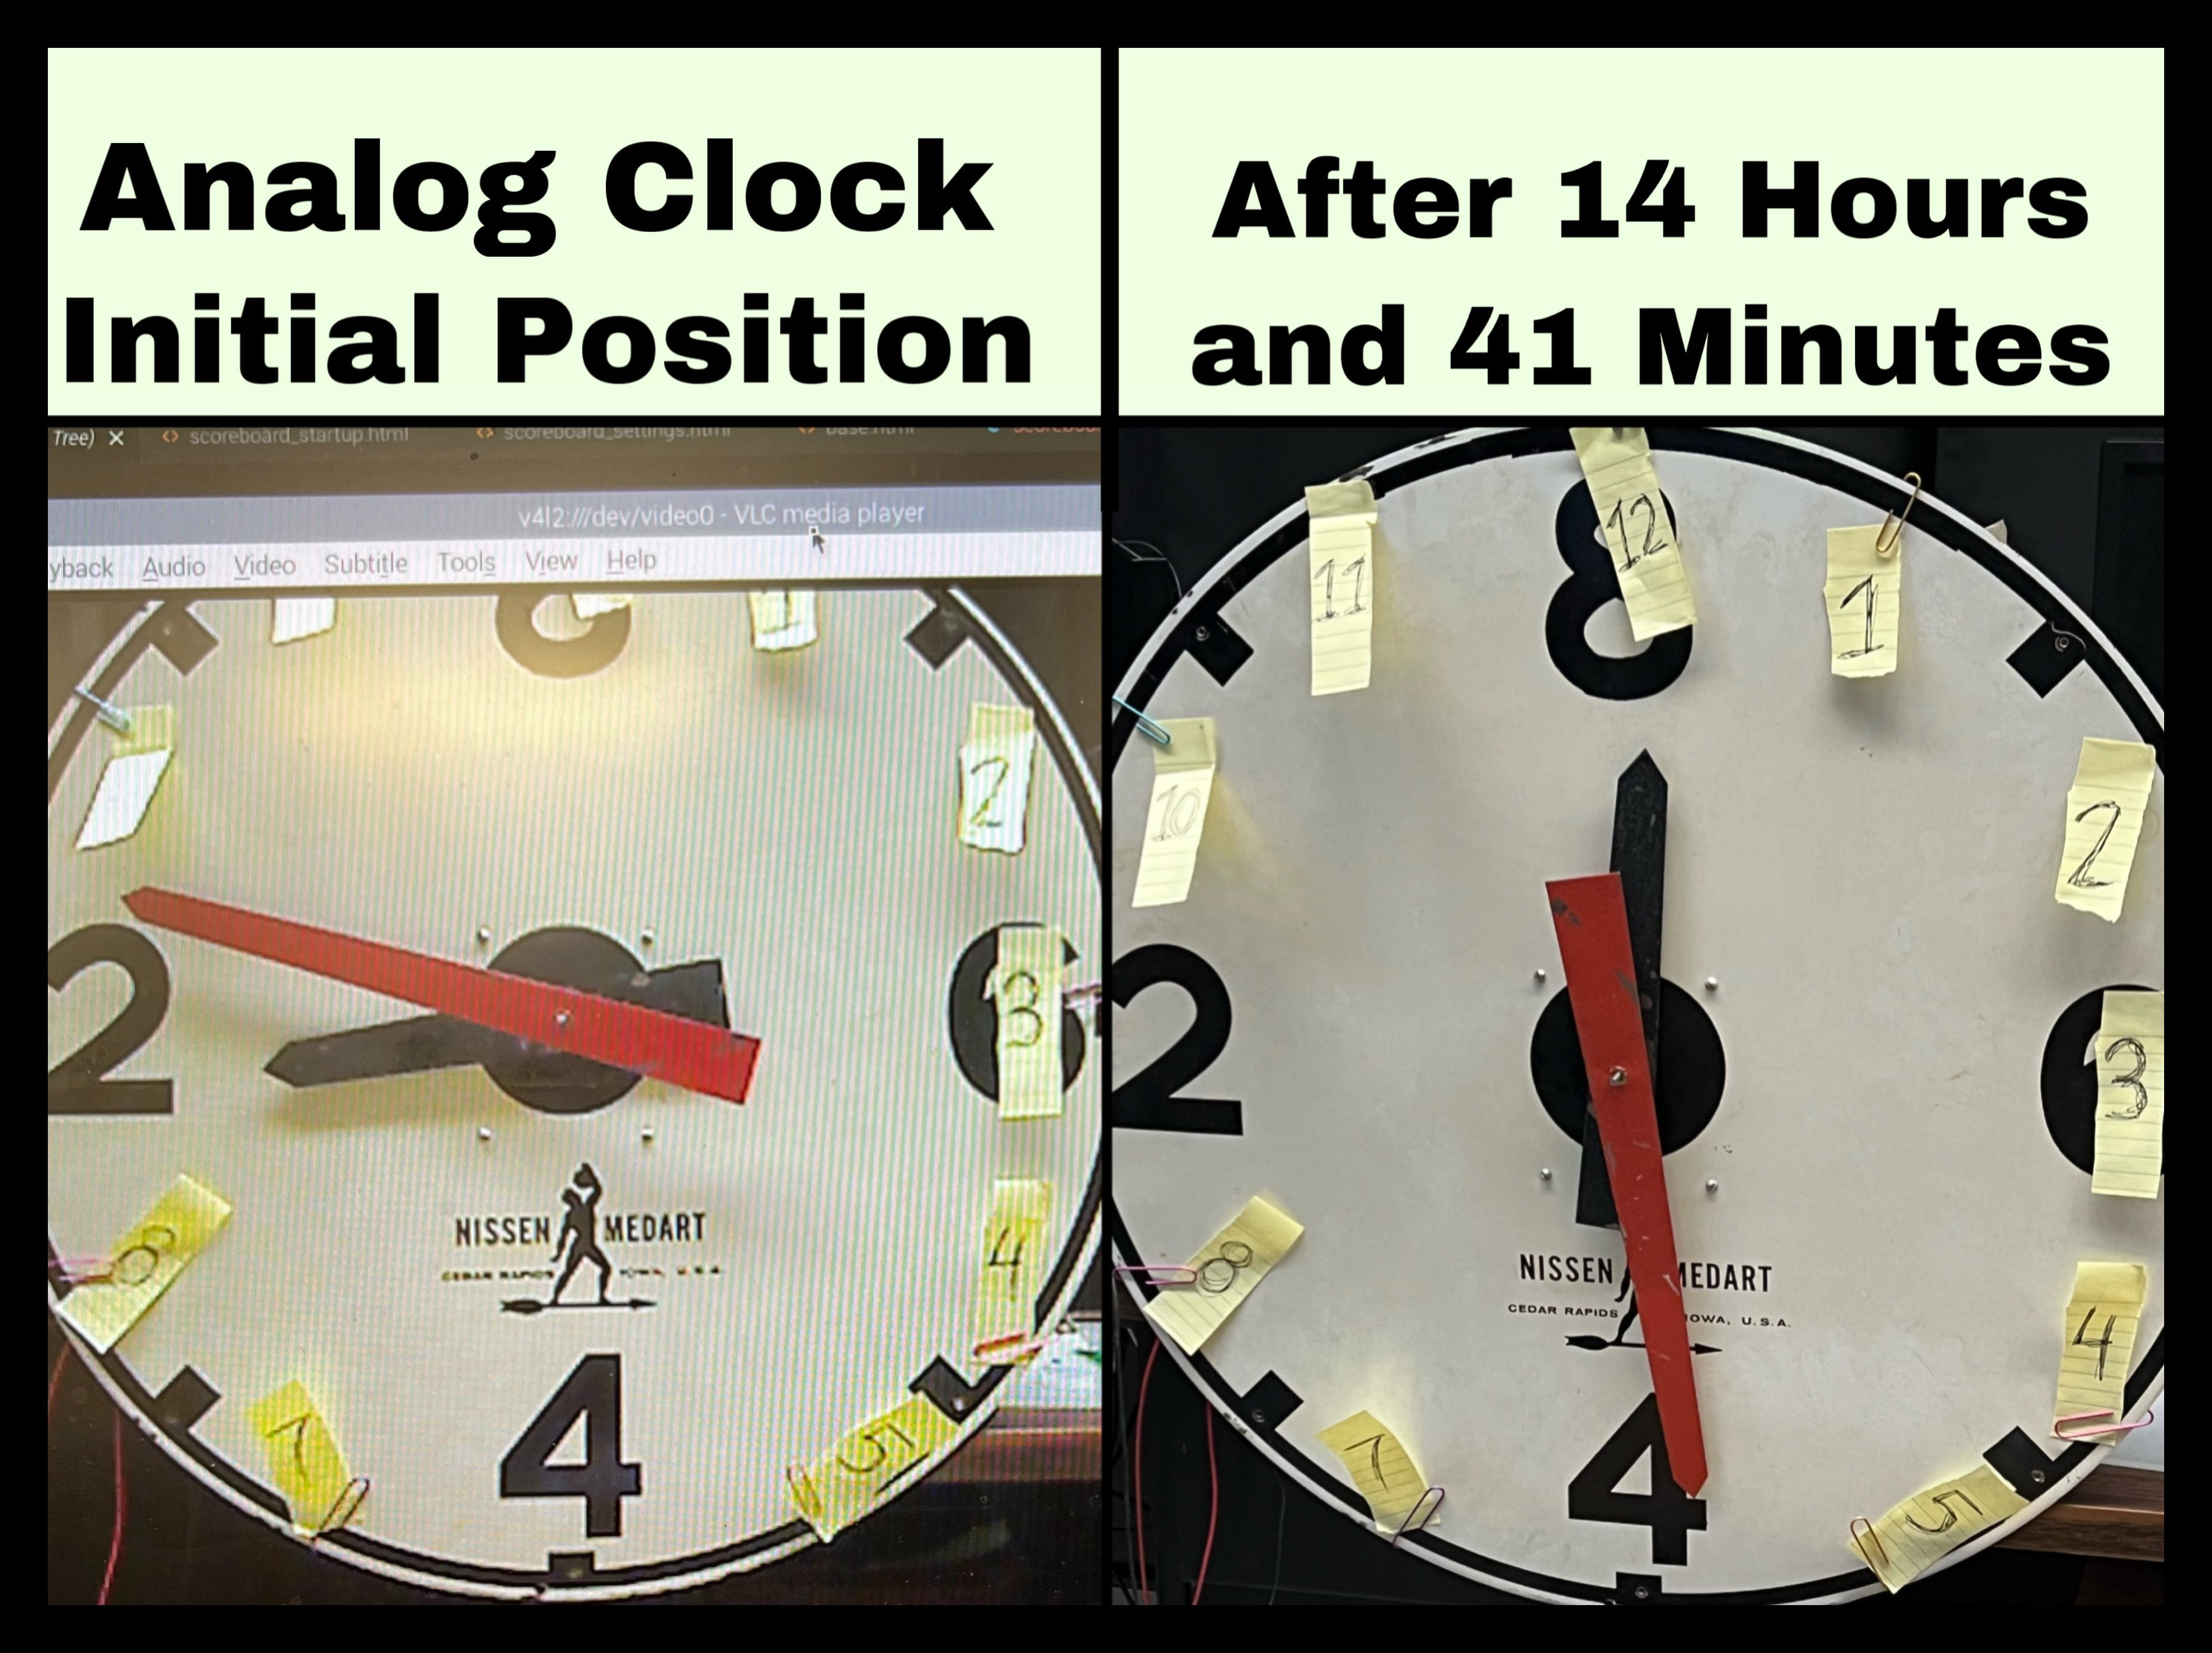
\includegraphics[width=5in]{analogTest1.jpg}
\caption{Analog Clock Hand positions Before and After 14 Hours and 41 Minutes}
\label{analogTest1}
\end{figure}

\begin{table}[h!]
    \caption{Tests of the Analog Clock Hand Ratios over Extended Periods of Time}
    \resizebox{\textwidth}{!}{%
    \begin{tabular}{l|c|c|c|}
    \cline{2-4}
     & \multicolumn{1}{l|}{\textbf{Actual Time}} & \multicolumn{1}{l|}{\textbf{\begin{tabular}[c]{@{}l@{}}Actual Analog \\ Clock Display Time\end{tabular}}} & \multicolumn{1}{l|}{\textbf{\begin{tabular}[c]{@{}l@{}}Expected Analog \\ Clock Display Time\end{tabular}}} \\ \hline
    \multicolumn{1}{|l|}{\multirow{2}{*}{\textbf{\begin{tabular}[c]{@{}l@{}}Test 1 Duration:\\ (14 Hrs and 41 Min)\end{tabular}}}} & 07:46PM & 08:47 & N/A \\ \cline{2-4} 
    \multicolumn{1}{|l|}{} & 10:27PM & 12:28 & 11:28 \\ \hline
    \multicolumn{1}{|l|}{\multirow{2}{*}{\textbf{\begin{tabular}[c]{@{}l@{}}Test 2 Duration:\\ (3 Hrs and 0 Min)\end{tabular}}}} & 01:35PM & 12:00 & N/A \\ \cline{2-4} 
    \multicolumn{1}{|l|}{} & 04:35PM & 03:00 & 03:00 \\ \hline
    \bottomrule
    \end{tabular}%
    }
\label{tab:analogTest}
\end{table}


Between Test 1 and Test 2, an adjustment was made in the clock hand ratio algorithm to eliminate the extra 4 ms delay every 27 seconds when there is an hour hand step. For Test 1 with a period of 14 hours and 41 minutes (or 52680 seconds), there would be an expected total error delay of 7.828 seconds, which would correspond to a delay of at most 4 steps of the total 1600 steps per revolution. However, that compounded 7.828 seconds of error is after over 14 hours of running. As will be discussed in Section \ref{future}, synchronization of the clock to an on-board RTC every several hours is a possible future improvement that could be made to further ensure any delay could not compound to a significant level. 

In addition, between Test 1 and Test 2, the hour hand's set-screw attachment to the shaft was adjusted to ease some tension within the gearbox that had lead to some slipping of the hand instead of smooth circular motion. 

Some of the error in position for Test 1 could have also been from the starting position of the clock hands. The starting analog clock position of 7:46 was not one that was best for ensuring accuracy of the hour hand position. The current clock face still has the original paint that only has 8 markings along the edge of the face. Hours like 12, 3, 6, and 9 are much easier to visually confirm the position of, while the other hour markers have to be estimated based on the markings that occur every $45^\circ$. In addition, with the minute being 46, the hour hand would need to be a large portion of the way towards the next hour. 

While Test 1 had issues, the results it provided were still relevant to testing the accuracy of the ratio by showing the general ratio and timing had accuracy of the minute hand and the hour hand. For the next test, the hands were started at the noon position. This would mean that, after the 3 hours elapsed, the clock hands would be expected to be at positions that were more easily verified with the existing markings. 

Test 2 showed that, with the slight adjustments made between tests to the software and mechanics, the accuracy was indeed to the minute. 

%TEST 2 analysis here%

% For the digital clock, the PCB will need to be fully incorporated once it arrives, and then tested to ensure proper functionality. 
In order to provide Ft. Fairfield with reliable electronics, and reliable, easily-installed replacements for the electronics should they fail, a custom PCB was incorporated into the scoreboard chassis. The PCB currently has a component selection flaw that has been manually revised, and future revisions of the PCB will address the component selection issue.

The separate components of this project (motors, motor drivers, microcontrollers, LCD drivers, etc.) function correctly currently while connected with wiring, but they are yet to be physically installed inside of the chassis. 
Installation in the chassis needs to be done to ensure that continues, especially with the chassis being made entirely of metal that functions as a ground for some circuitry. 

The current GUI can be seen in Figure \ref{currGUI} and \ref{currGUICalli}. On both screens the current system time, received from \textbf{datetime} in the \textbf{Python} script, is displayed, and updated without requiring a page refresh. 

\begin{figure}[H]
\centering
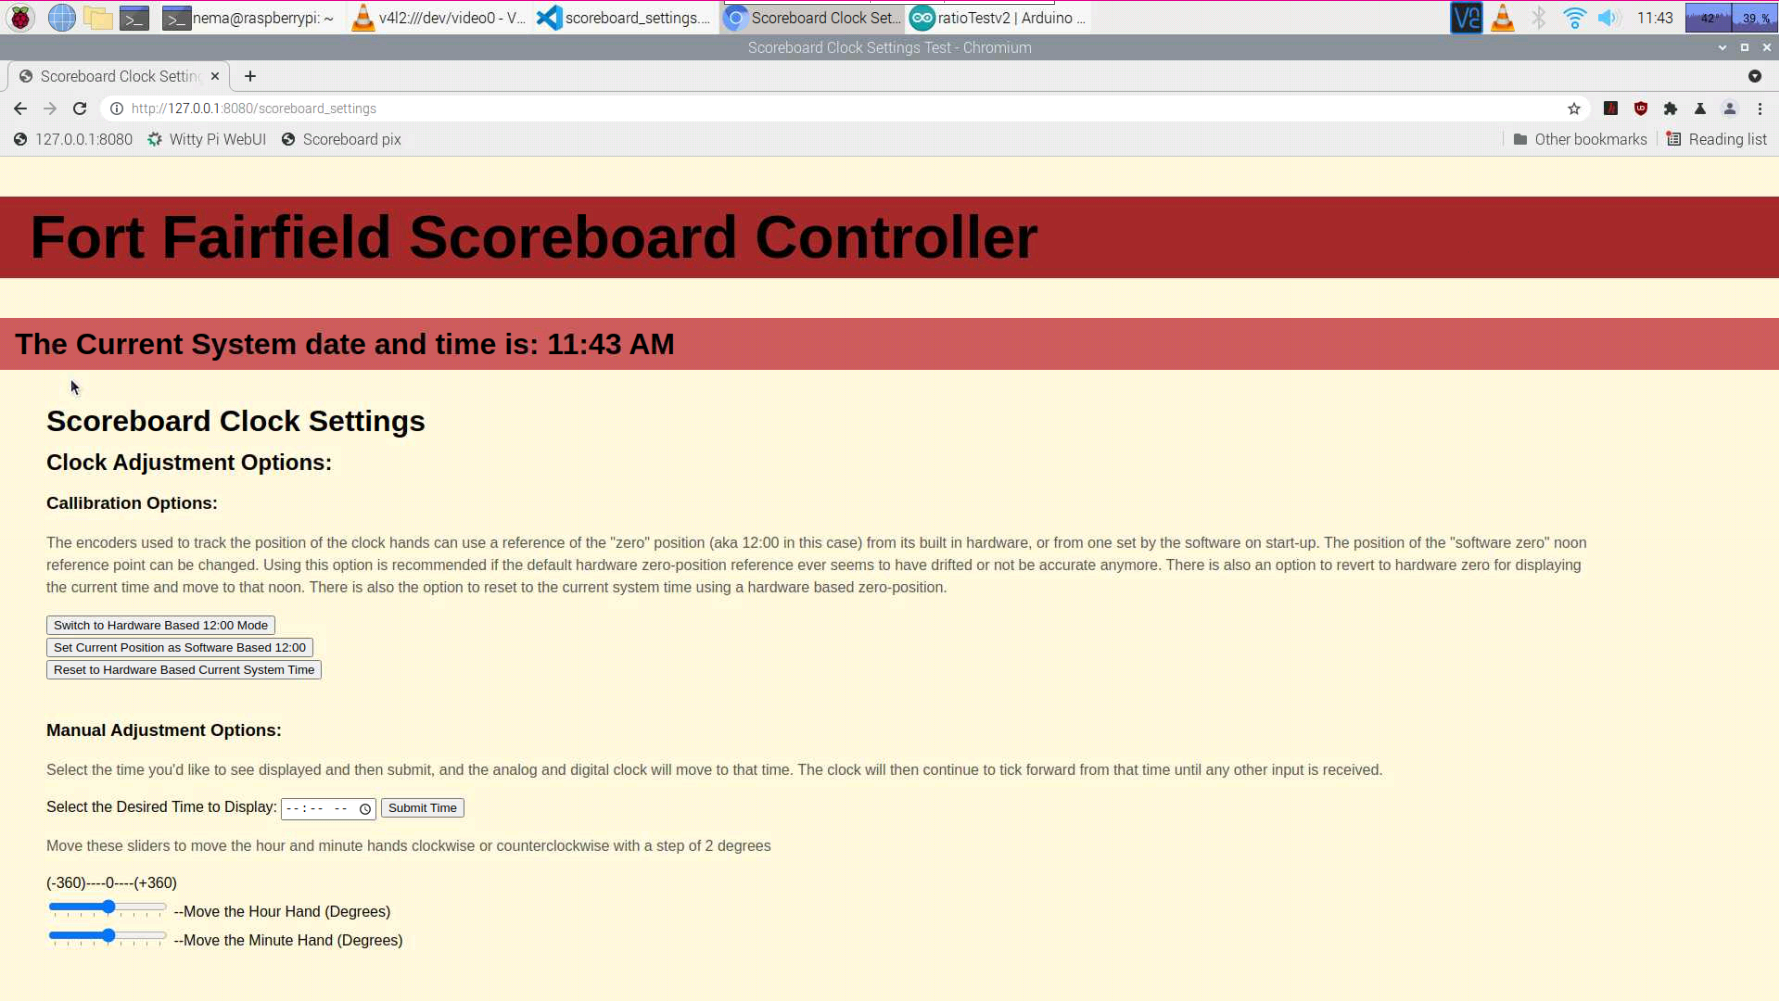
\includegraphics[width=6.5in]{main_gui.PNG}
\caption{Current Flask managed Graphical User Interface (GUI) of the "Advanced Settings" Mode}
\label{currGUI}
\end{figure}

When the \textbf{Python} script first runs, the user is brought to the Calibration screen of the GUI. That can be seen in Figure \ref{currGUICalli}. The user is prompted to enter the time that the hands of the clock appear to be currently displaying, and the hands then move to the position for noon to set the software-based zero of the rotary encoders at that position. This provides user input that controls the clocks, meeting the contract specifications. Then, the hands move to the current system time. The user can then select the button to "Go to Scoreboard Clock Advanced Controls", which would navigate them to the next screen: Figure \ref{currGUI}.

% need to ensure it works while isntalled and is secure
\begin{figure}[H]
\centering
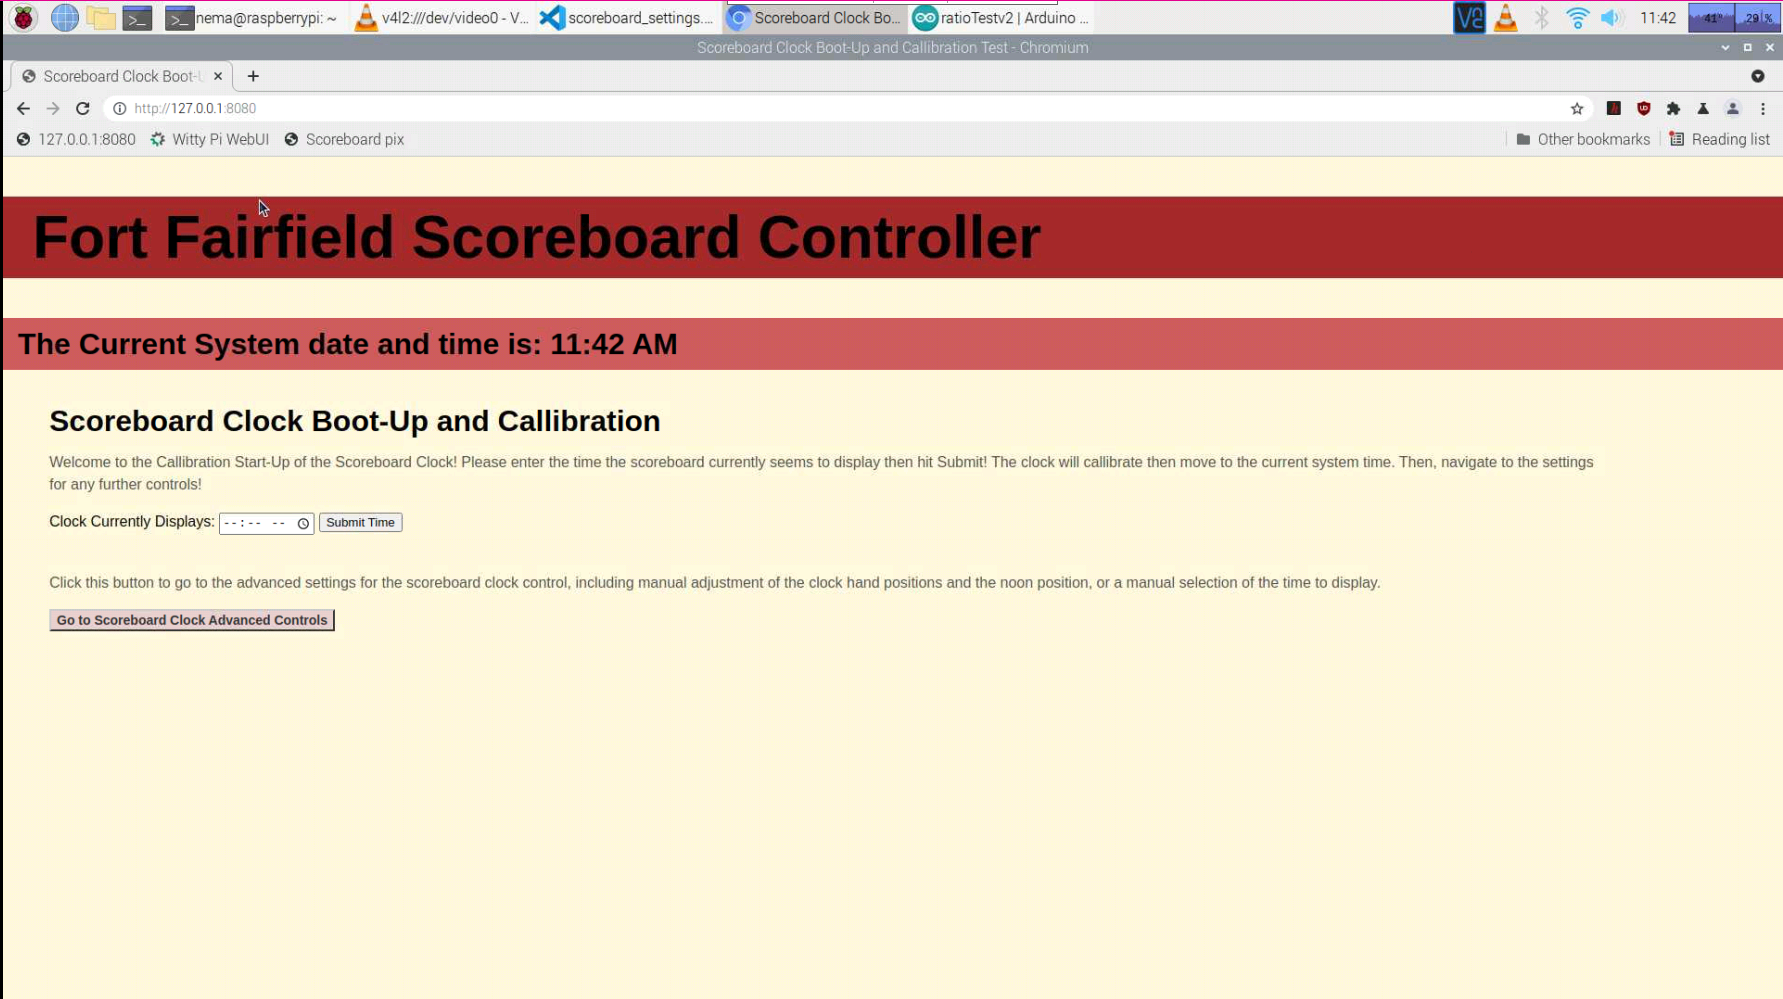
\includegraphics[width=6.5in]{callibration_screen.PNG}
\caption{Current Flask managed Graphical User Interface (GUI) of the "Initial Calibration" Mode}
\label{currGUICalli}
\end{figure}.

% talk through interface currently and what each thing means

Here, the user has more options of user input that can control the clock, as per the contract specifications. A description is included for each of the options to make the function of the options available clearer to the user.


\subsection{Future Improvements}
\label{future}

In this section, improvements deemed as viable and valuable to the quality of the scoreboard clock are enumerated. These will take the form of near future improvements, while others are possible far future improvements. Note that these will not all be completed before the delivery of the scoreboard to the Rec. Dept. of Ft. Fairfield, before the end of April 2022.

%While the mechanical portions of the projects were completed to the best of the team's ability, but still, there remain portions of the mechanical build that 
A desktop launcher for the \textbf{Python} script and GUI is intended to be added to make the control of the device more user friendly. There is also intent to create scheduled tasks that will run the time synchronization script from the connected on-board RTC module (WittyPi3Mini) to ensure accuracy of time. This would be run at the very least during the hours of midnight to 4am where it could be expected that any necessary minor adjustments of the clock hand positions would be likely to not be noticed. More frequent synchronization of the system time to compensate for any minor delay of the clock hands will also be explored. 

Under ideal conditions, Ft. Fairfield's scoreboard would be shipped with a multiplexing controller board that was soldered completely using surface-mount components. The first revision of the PCB has through-hole headers soldered by hand, in addition to the problematic selection the FS8205A NMOS transistors which multiplex the connection to ground. The dual transistor package has a common drain for the two transistors. As such, regardless of which connection to ground is toggled on this MOSFET array, electrically toggling either gate of the MOSFET array wires two LED arrays in parallel. This configuration is undesirable because the display multiplexing configuration relies on exactly one LED matrix being selected per character displayed. This can be solved by finding a transistor array with the same SOT-23-6 package and pinout.

Having independent stepper motors for each hand instead of a true gear box allows for options of future development of different modes such as a scoreboard mode a user could switch between. The MCUs are able to both be flashed from the RPi, so future developers could make their own software inclusions using the same hardware. 

Other future improvements could include a speaker connected where the buzzer once was internally for various applications. 


%Rough draft content --v
%Improvements to be implemented in the future:\\
%- have the webpage be automatically updated at least once every minute so the  time displayed on the web page is accurate and to ensure that any manual movement of the hands is reset back to desired time, similarly, add a user input button as a "move to current system time", make it look a little nicer with instructions and explanations built in\\
%- 3D printed structure  for the stepper motor box to keep encoders in place, and ensure it doesn't \\
%- add a startup script for the analog clock to calibrate on boot up before the web page is run, have it move to HW based noon, and set that as the SW noon, then move to current time, then have the web page boot up for the user, or have the GUI display a message of: Calibrating Clock (Starting at 12:00, moving to current time, Ready!) then moving to the GUI capable of accepting user input\\
%- having the launcher for the \textbf{Flask} \textbf{Python} script run automatically when the RPi boots up. (Currently have it able to be accessed externally using an ssh connection)\\
%- using WittyPi, using it without giving elevated permissions \\

%possible improvements for the far future


\section{Conclusion}
\label{conclusion}

The design process of the vintage scoreboard with analog and digital clocks has been described in this report. 
The construction process is still actively occurring, but the progress as of the writing of this report has been detailed as well. 
The mechanical, hardware, and software components were all discussed. 
As of writing this report, the specifications of user input being able to control the clocks with a GUI, and the project being controlled by a Raspberry Pi single-board computer have been met. 
Also as specified, the board receives power from a 120 $V_{rms}$ wall outlet, has networking capability via Wi-Fi, and uses local time for clock synchronization. 
While the clock hands are able to be moved to display the analog time and the LED arrays are capable of displaying numbers, currently a time display with accuracy to the minute has not been achieved. 

This project provides not only insight into the creative methods of electrical engineering from decades ago, but also provides a look into modern issues of technological waste and the life cycle of technology. 
This project incorporates many aspects of the engineering curriculum, and blurs the line between several engineering disciplines to include aspects of Electrical, Computer, and Mechanical Engineering. 
With aspects of engineering across various times and disciplines, this project provides a fitting conclusion to the undergraduate Electrical and Computer curriculum at the University of Maine while also preserving a piece of history for Fort Fairfield.


\newpage
\appendix
\titlespacing*{\section}{0pt}{0pt}{-8pt}

\section{Project Contract}
\label{appendix:contract}
% Title and author
\setlength{\parskip}{0.5em}

\singlespacing
\LARGE{{ \textbf{Vintage Scoreboard with Digital and Analog Clocks }}}\\
\large{\author{Alessandra DiFilippo (CE) \\ 
Miles Martin (CE) }
\date{\today}}
%\thispagestyle{empty}

\setlength{\parskip}{0.5em}

\title{\textbf{Description}}

A vintage basketball scoreboard will be revitalized with new functionality in this project. 
The clock face on the left will display the accurate analog time and an array of light-emitting diodes (LEDs) on the right will display the accurate digital time. 
The device will be connected to and controlled by a Raspberry Pi connected to a wireless network. 
The wireless network connection will facilitate a number of functions, such as time synchronization of the on-board real-time clock (RTC) to set it to Eastern Standard Time (EST) via the Network Time Protocol (NTP). 
Remote management of the scoreboard's hardware will also be possible through the wireless connection.
% Removed note about animations
The device will be powered from a 120 V$_{rms}$ wall outlet. 
A graphical user interface (GUI) will allow a user to program a variety of functions, including an LED matrix display and analog clock control.
% The display will be programmable so that animations can play on an internal or external trigger. 
% Also, in software, debug mode may be enabled, which will allow for the display of up to 15 error codes on the game quarter indication lights. 
% The error codes will be expressed in binary.
% The unit is also equipped with a buzzer, which will be re-configurable and programmable by the user via the GUI.

\textbf{Inputs}
\begin{itemize}
  \setlength\itemsep{0.15em}
  \item Power from 120 V$_{rms}$ wall outlet
  % \item Real-time clock synchronize to Eastern Standard Time via over Wi-Fi
  \item Local time for internal clock synchronization
  \item Networking capability via Wi-Fi
  \item User input via GUI
\end{itemize}

\textbf{Outputs}
\begin{itemize}
  \item Movement of analog clock hands
  \item Digital time display using array of LEDs
\end{itemize}

\textbf{Specifications}

\begin{itemize}
  \item User input can control/program the clocks
  \item Controlled by Raspberry Pi single-board computer
  \item Display current time on both the analog and digital clock with accuracy to the minute
  
\end{itemize}


\newcommand\signature[1]{% Name; Department
\noindent\begin{minipage}{5cm}
    \noindent\vspace{1cm}\par
    \noindent\rule{6cm}{1pt}\par
    \noindent\textbf{#1}
\end{minipage}}

\signature{Alessandra DiFilippo} \hfill \signature{Date of signature}

\signature{Miles Martin}\hfill\signature{Date of signature}

\newpage

\section{Parts List}
\label{appendix:parts}
% Please add the following required packages to your document preamble:
% \usepackage{graphicx}
\begin{table}[htp]
\resizebox{\textwidth}{!}{%
\begin{tabular}{|lrlrr|}
\hline
\multicolumn{1}{|c|}{\textbf{Item}} & \multicolumn{1}{c|}{\textbf{Qty}} & \multicolumn{1}{c|}{\textbf{Description}} & \multicolumn{1}{c|}{\textbf{\begin{tabular}[c]{@{}c@{}}Cost \\ (\$ Per Unit)\end{tabular}}} & \multicolumn{1}{c|}{\textbf{\begin{tabular}[c]{@{}c@{}}Extended \\ Cost (\$)\end{tabular}}} \\ \hline
\multicolumn{5}{|c|}{\textbf{Mechanical \& Non-Eletronic Hardware and Components}} \\ \hline
\multicolumn{1}{|l|}{34-Teeth Pinion Gear for 5mm shaft} & \multicolumn{1}{r|}{3} & \multicolumn{1}{l|}{34-T Pinion Gear (1.0 metric pitch) and 20 Degree Pressure Angle} & \multicolumn{1}{r|}{\$8.39} & \$25.17 \\ \hline
\multicolumn{1}{|l|}{4mm to 5mm Shaft Coupling} & \multicolumn{1}{r|}{2} & \multicolumn{1}{l|}{4mm to 5mm Shaft Coupling 25mm Length, 18mm Diameter} & \multicolumn{1}{r|}{\$4.15} & \$8.29 \\ \hline
\multicolumn{1}{|l|}{5mm to 6mm Shaft Coupling} & \multicolumn{1}{r|}{5} & \multicolumn{1}{l|}{Flexible Couplings 5mm to 6mm  Aluminum Alloy Joint} & \multicolumn{1}{r|}{\$1.94} & \$9.68 \\ \hline
\multicolumn{1}{|l|}{Red BA9s Lightbulb} & \multicolumn{1}{r|}{110} & \multicolumn{1}{l|}{\begin{tabular}[c]{@{}l@{}}BA9s LED Landscape Light Bulb BA9s Retrofit - 5 Lumens \\ Red 180 Degree 12VAC/DC\end{tabular}} & \multicolumn{1}{r|}{\$0.96} & \$105.60 \\ \hline
\multicolumn{1}{|l|}{Molex Pin Crimp Connectors} & \multicolumn{1}{r|}{100} & \multicolumn{1}{l|}{CONN SPLIT PIN 14-20AWG CRMP TIN} & \multicolumn{1}{r|}{\$0.07} & \$7.00 \\ \hline
\multicolumn{1}{|l|}{Stepper Motor Mounting Brackets} & \multicolumn{1}{r|}{6} & \multicolumn{1}{l|}{Nema 17 Stepper Motor Mounting Brackets with M3 Screws} & \multicolumn{1}{r|}{\$2.50} & \$15.00 \\ \hline
\multicolumn{1}{|l|}{\begin{tabular}[c]{@{}l@{}}Brass Shaft \\ Mounting kit\end{tabular}} & \multicolumn{1}{r|}{1} & \multicolumn{1}{l|}{\begin{tabular}[c]{@{}l@{}}M2 M3 Hex Male Female Brass Standoff Hexagon Threaded Stud \\ Board Pillar Mounting Spacer Bolt Screw Nut Assortment Kit 240Pcs\end{tabular}} & \multicolumn{1}{r|}{\$12.90} & \$12.90 \\ \hline
\multicolumn{1}{|l|}{5mm Diameter Magnets} & \multicolumn{1}{r|}{200} & \multicolumn{1}{l|}{Deryun Small Magnets, 200 Pack} & \multicolumn{1}{r|}{\$0.05} & \$10.00 \\ \hline
\multicolumn{1}{|l|}{Translucent Red PLA Filament} & \multicolumn{1}{r|}{1} & \multicolumn{1}{l|}{1.75mm PLA Filament 1kg / 2.2lb for 3D Printers, Translucent Red} & \multicolumn{1}{r|}{\$22.95} & \$22.95 \\ \hline
\multicolumn{1}{|l|}{48T, 14.5 PA Brass Gear} & \multicolumn{1}{r|}{2} & \multicolumn{1}{l|}{Tradeship Solid Brass 48 Pitch 48 Teeth 14.5 PA Gears} & \multicolumn{1}{r|}{\$12.80} & \$25.60 \\ \hline
\multicolumn{1}{|l|}{Black Tubing} & \multicolumn{1}{r|}{1} & \multicolumn{1}{l|}{4" Diameter Snap Coupling (24/BG), (Cut in half at diameter)} & \multicolumn{1}{r|}{\$5.98} & \$5.98 \\ \hline
\multicolumn{5}{|c|}{\textbf{Programmable Hardware}} \\ \hline
\multicolumn{1}{|l|}{TMC2209 SilentStepStick} & \multicolumn{1}{r|}{2} & \multicolumn{1}{l|}{TMC2209 SilentStepstick Stepper Driver Board} & \multicolumn{1}{r|}{\$16.03} & \$32.06 \\ \hline
\multicolumn{1}{|l|}{Tiva C} & \multicolumn{1}{r|}{1} & \multicolumn{1}{l|}{TI ARM® Cortex®-M4F Based MCU TM4C123G LaunchPad™} & \multicolumn{1}{r|}{\$0.00} & \$0.00 \\ \hline
\multicolumn{1}{|l|}{ATmega Microcontroller} & \multicolumn{1}{r|}{1} & \multicolumn{1}{l|}{ELEGOO MEGA R3 Board ATmega, Compatible with Arduino IDE} & \multicolumn{1}{r|}{\$22.99} & \$22.99 \\ \hline
\multicolumn{1}{|l|}{Arduino Nano} & \multicolumn{1}{r|}{2} & \multicolumn{1}{l|}{Arduino Nano with ATmega328 base} & \multicolumn{1}{r|}{\$0.00} & \$0.00 \\ \hline
\multicolumn{1}{|l|}{Arduino Uno} & \multicolumn{1}{r|}{1} & \multicolumn{1}{l|}{Arduino Uno ATmega328P microcontroller board} & \multicolumn{1}{r|}{\$0.00} & \$0.00 \\ \hline
\multicolumn{1}{|l|}{Raspberry Pi 4B} & \multicolumn{1}{r|}{1} & \multicolumn{1}{l|}{Raspberry 4 Model B} & \multicolumn{1}{r|}{\$0.00} & \$0.00 \\ \hline
\multicolumn{1}{|l|}{RPi RTC and Power Management} & \multicolumn{1}{r|}{1} & \multicolumn{1}{l|}{Witty Pi 3 Mini- RTC \& Power Management Board for Raspberry Pi} & \multicolumn{1}{r|}{\$19.95} & \$19.95 \\ \hline
\multicolumn{5}{|c|}{\textbf{PCB Components}} \\ \hline
\multicolumn{1}{|l|}{C2685142} & \multicolumn{1}{r|}{2} & \multicolumn{1}{l|}{Liansheng PH-00205 1A Straight Square Pins 1.7mm 6mm} & \multicolumn{1}{r|}{\$0.56} & \$1.12 \\ \hline
\multicolumn{1}{|l|}{C261283} & \multicolumn{1}{r|}{22} & \multicolumn{1}{l|}{\begin{tabular}[c]{@{}l@{}}Tak Cheong 2SK3019 0V 100mA 8$\Omega$ @4V,10mA 150mW \\ 1.5V@100$\mu$A N Channel SOT-523 MOSFETs\end{tabular}} & \multicolumn{1}{r|}{\$0.03} & \$0.66 \\ \hline
\multicolumn{1}{|l|}{C699284} & \multicolumn{1}{r|}{11} & \multicolumn{1}{l|}{\begin{tabular}[c]{@{}l@{}}Yangzhou Yangjie Elec Tech YJS2301A  20V 3.7A 49m$\Omega$ @4.5V,3.4A \\ 1.3W 620mV@250uA 65pF@10V 2 P-Channel 550pF@10V \\ 4.3nC@4.5V -55℃$\sim$+150℃@(Tj) SOT-23-6L MOSFETs\end{tabular}} & \multicolumn{1}{r|}{\$0.07} & \$0.77 \\ \hline
\multicolumn{1}{|l|}{C908265} & \multicolumn{1}{r|}{2} & \multicolumn{1}{l|}{\begin{tabular}[c]{@{}l@{}}FUXINSEMI FS8205A 20V 6A 18m$\Omega$ @4.5V,6A 1.5W 1.2V@250uA \\ 125pF@8V 2 N-Channel 800pF@8V 11nC@4.5V -55℃$\sim$+150℃@(Tj) \\ SOT-23-6L MOSFETs\end{tabular}} & \multicolumn{1}{r|}{\$0.07} & \$0.14 \\ \hline
\multicolumn{1}{|l|}{C520866} & \multicolumn{1}{r|}{22} & \multicolumn{1}{l|}{\begin{tabular}[c]{@{}l@{}}KOA Speer Elec RN731JTTD1003B25 ±0.1\% 63mW ±25ppm/℃ \\ 100k$\Omega$ 0603 Chip Resistor - Surface Mount\end{tabular}} & \multicolumn{1}{r|}{\$0.15} & \$3.30 \\ \hline
\multicolumn{1}{|l|}{C489152} & \multicolumn{1}{r|}{4} & \multicolumn{1}{l|}{\begin{tabular}[c]{@{}l@{}}KEXIN KMP1340-079 50V -65℃$\sim$+150℃@(Tj) 250mW \\ 800mV@10mA 100ns 10$\mu$A@50V SOD-523 Switching Diode\end{tabular}} & \multicolumn{1}{r|}{\$0.11} & \$0.44 \\ \hline
\multicolumn{1}{|l|}{C706865} & \multicolumn{1}{r|}{1} & \multicolumn{1}{l|}{\begin{tabular}[c]{@{}l@{}}250V 3A Shrouded Square Pins 2.5mm 6mm -40℃$\sim$+105℃ \\ 1 2 2.54mm Black 1x2P Plugin,P=2.54mm Pin Headers ROHS\end{tabular}} & \multicolumn{1}{l|}{} & 0 \\ \hline
\multicolumn{5}{|c|}{\textbf{Other Hardware \& Electronics}} \\ \hline
\multicolumn{1}{|l|}{2x20 Adafruit GPIO Header} & \multicolumn{1}{r|}{1} & \multicolumn{1}{l|}{GPIO Stacking Header for Pi A+/B+/Pi 2/Pi 3 - Extra-long 2x20 Pins} & \multicolumn{1}{r|}{\$2.50} & \$2.50 \\ \hline
\multicolumn{1}{|l|}{RPi Power Supply Unit} & \multicolumn{1}{r|}{1} & \multicolumn{1}{l|}{Raspberry Pi 4 Model B Official PSU, USB-C, 5.1V, 3A, US Plug} & \multicolumn{1}{r|}{\$9.81} & \$9.81 \\ \hline
\multicolumn{1}{|l|}{Stepper Motors} & \multicolumn{1}{r|}{2} & \multicolumn{1}{l|}{Stepper Motor Hybrid Bipolar 12 V} & \multicolumn{1}{r|}{\$16.85} & \$33.70 \\ \hline
\multicolumn{1}{|l|}{Meanwell AC/DC 12V Converter} & \multicolumn{1}{r|}{1} & \multicolumn{1}{l|}{AC/DC CONVERTER 12V 25W} & \multicolumn{1}{r|}{\$12.30} & \$12.30 \\ \hline
\multicolumn{1}{|l|}{USB WiFi module (2.4GHz)} & \multicolumn{1}{r|}{1} & \multicolumn{1}{l|}{USB WIFI MODULE W/ANT 802.11B/G/N with external antenna} & \multicolumn{1}{l|}{} & 0 \\ \hline
\multicolumn{1}{|l|}{Hall Effect Sensors} & \multicolumn{1}{r|}{20} & \multicolumn{1}{l|}{A3144/OH3144/44E/AH3144E Hall Effect Sensor Magnetic Detector} & \multicolumn{1}{r|}{\$0.40} & \$8.00 \\ \hline
\multicolumn{1}{|l|}{Rotary Encoder} & \multicolumn{1}{r|}{3} & \multicolumn{1}{l|}{Bourns Rotary Encoder, Mechanical 128 PPR Binary (Absolute)} & \multicolumn{1}{r|}{\$8.86} & \$26.58 \\ \hline
\multicolumn{1}{|l|}{64GB MicroSD Card} & \multicolumn{1}{r|}{1} & \multicolumn{1}{l|}{Lexar 64 GB MicroSDHC UHS-I Card with SD Adapter} & \multicolumn{1}{r|}{\$19.99} & \$19.99 \\ \hline
\end{tabular}%
}
\end{table}

\newpage
\section{Project Schematics}
\label{appendix:schematics}

\titlespacing*{\chapter}{0pt}{0pt}{-20pt}


\begin{figure}[h!]
    \centering
    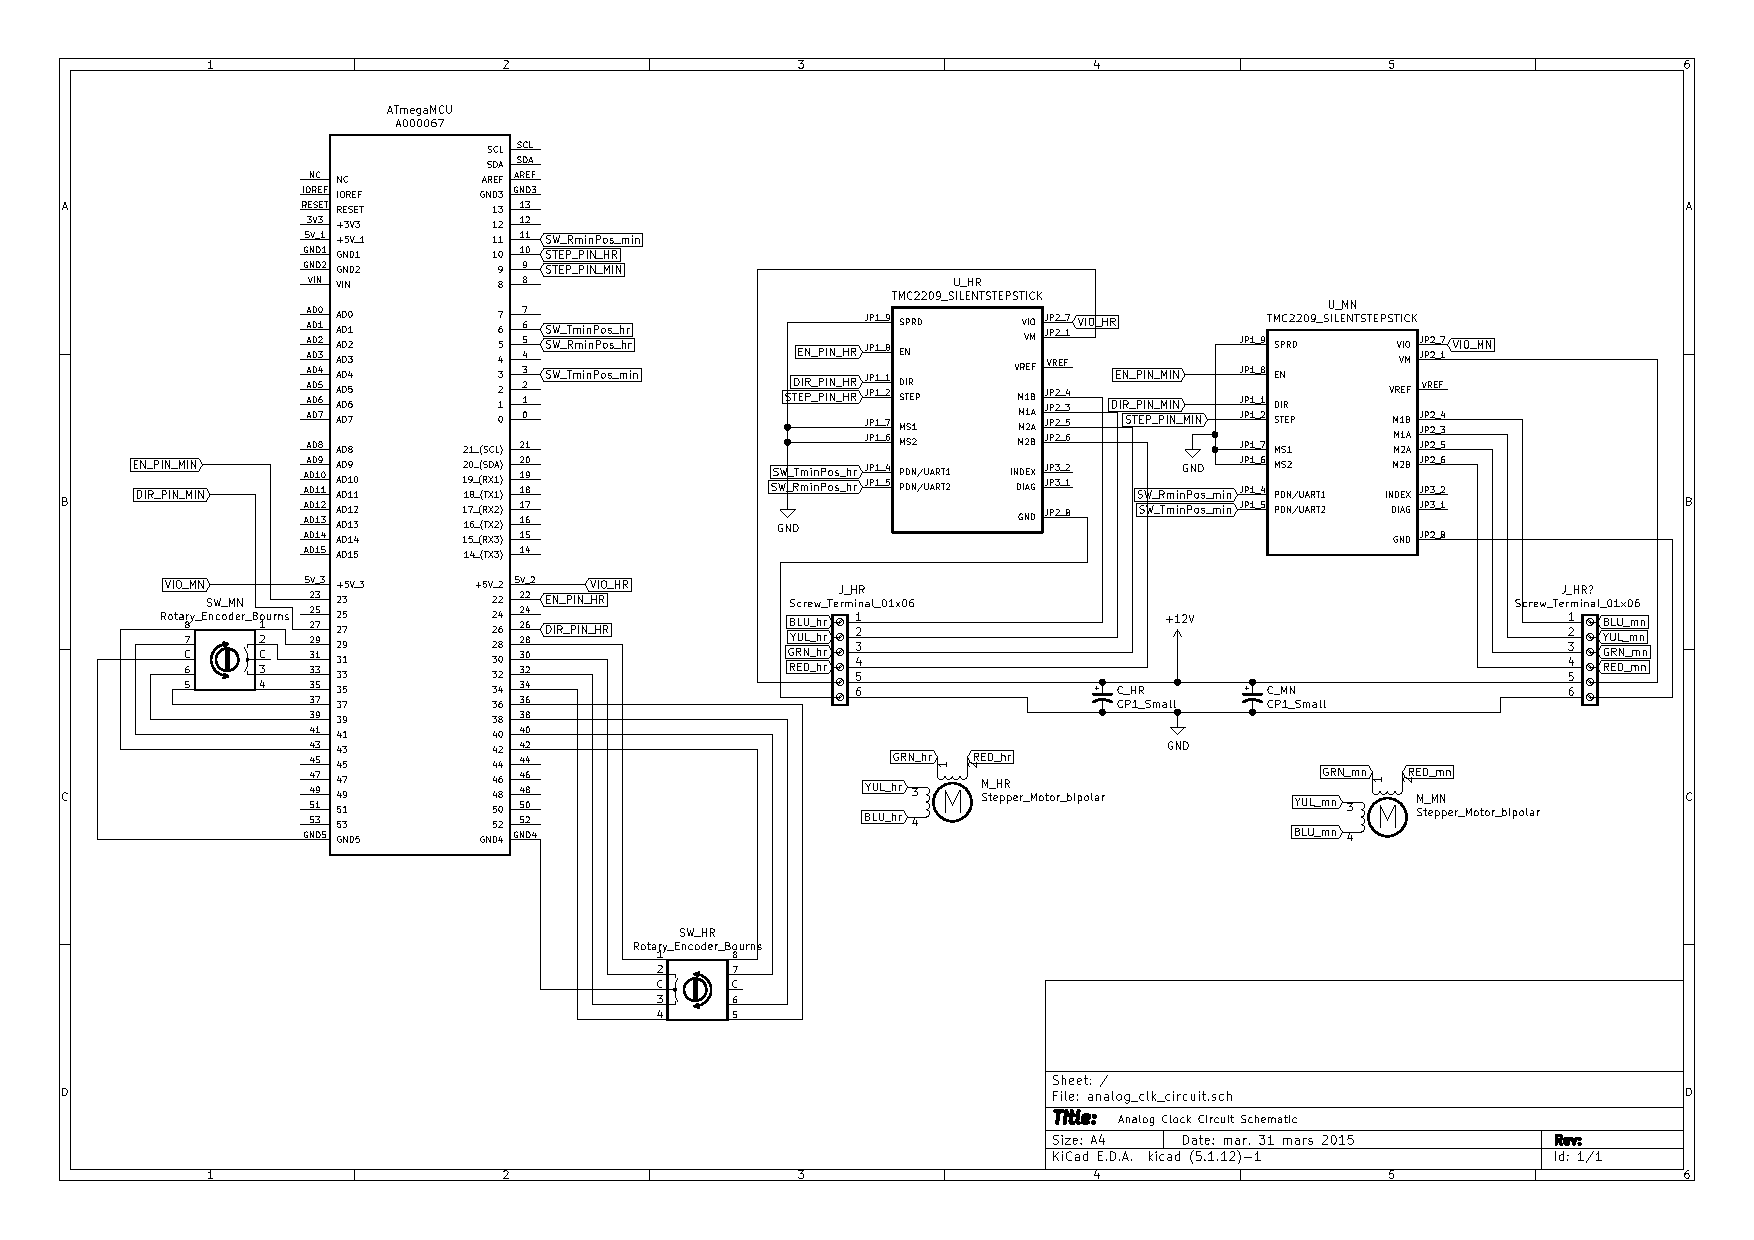
\includepdf[pages=-,scale=0.835,angle=90]{analog_clk_circuit.pdf}
    \rotcaption{Schematic of Analog Clock Circuitry and Hardware}
    %\rotcaption{Schematic of Analog Clock Circuitry and Hardware}[b]
\end{figure}

\newpage

\begin{figure}[h!]
 \centering
  %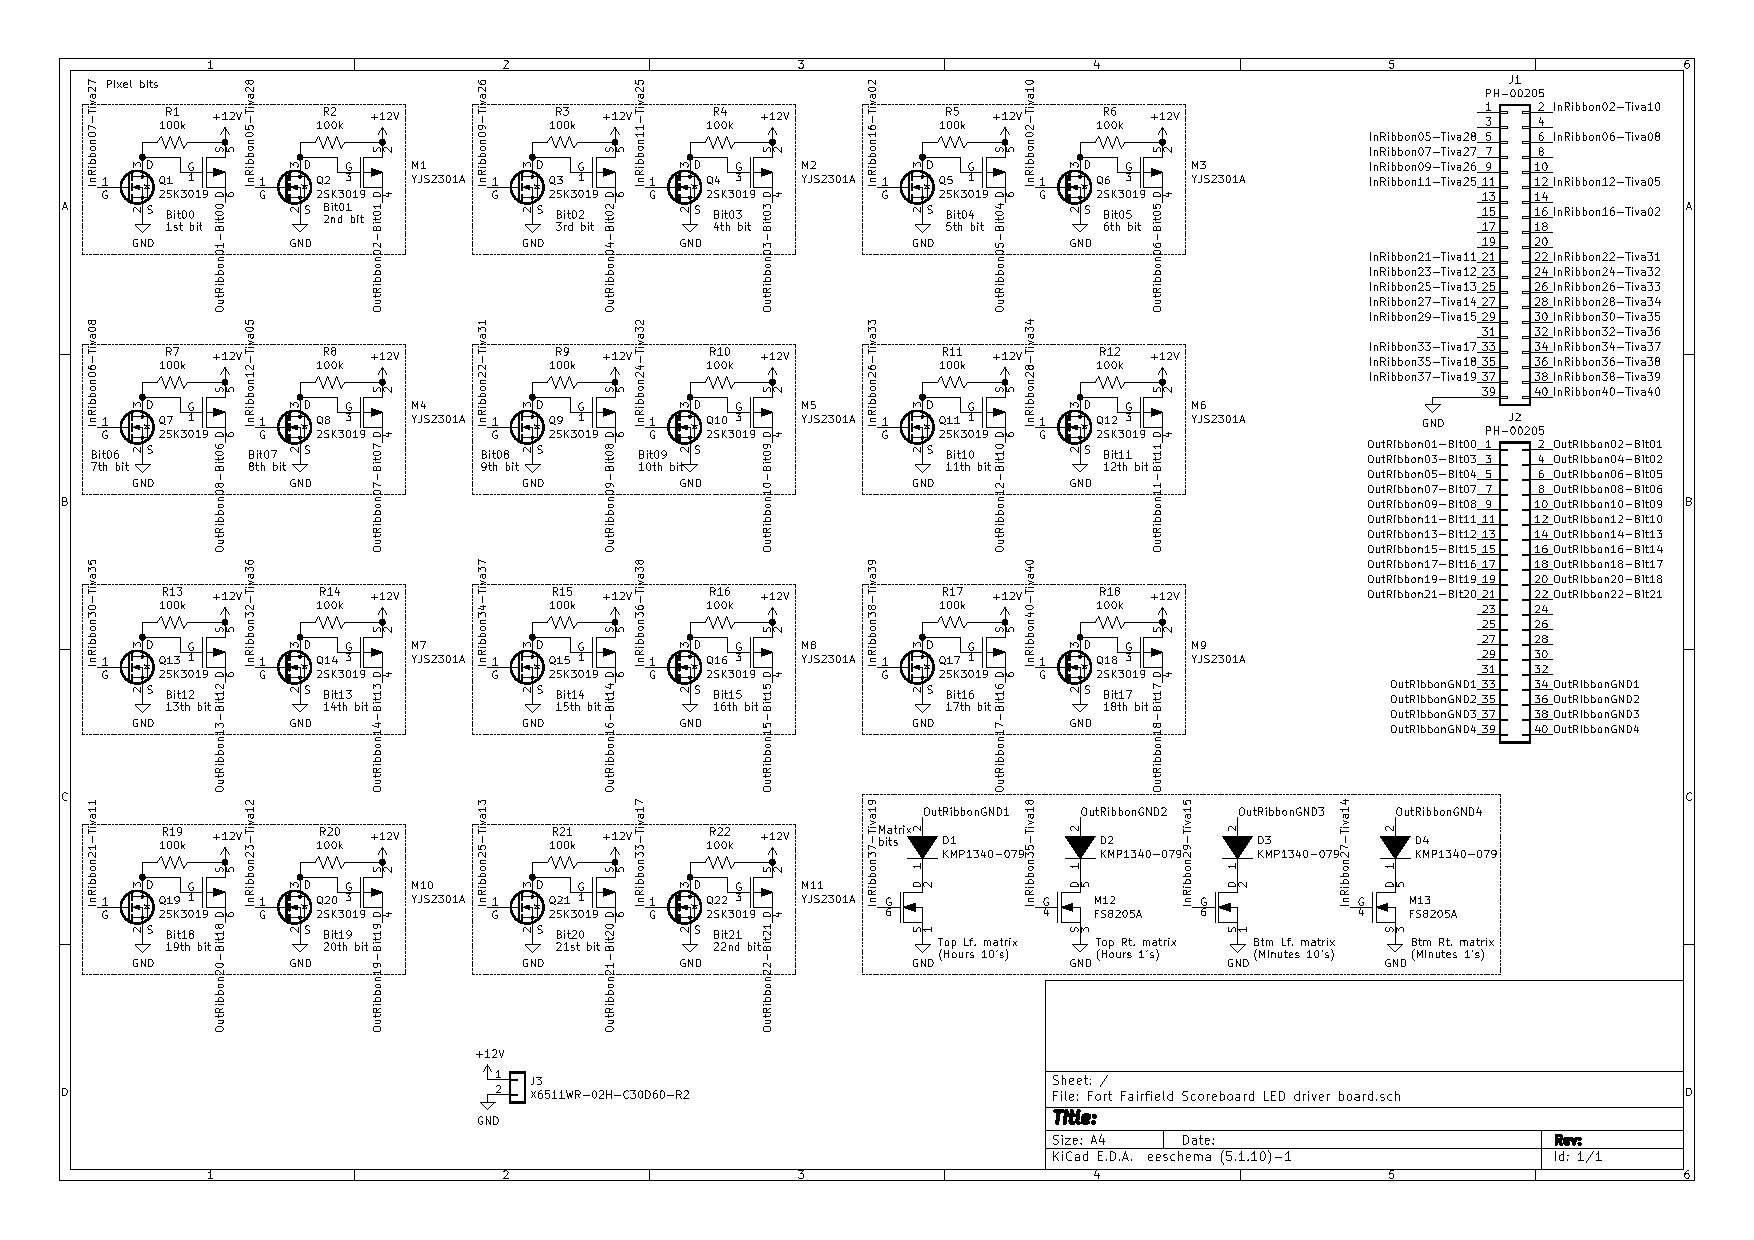
\includegraphics[scale=1,angle=-90]{evidence_createSchematics_1_LEDMuxer.pdf}
  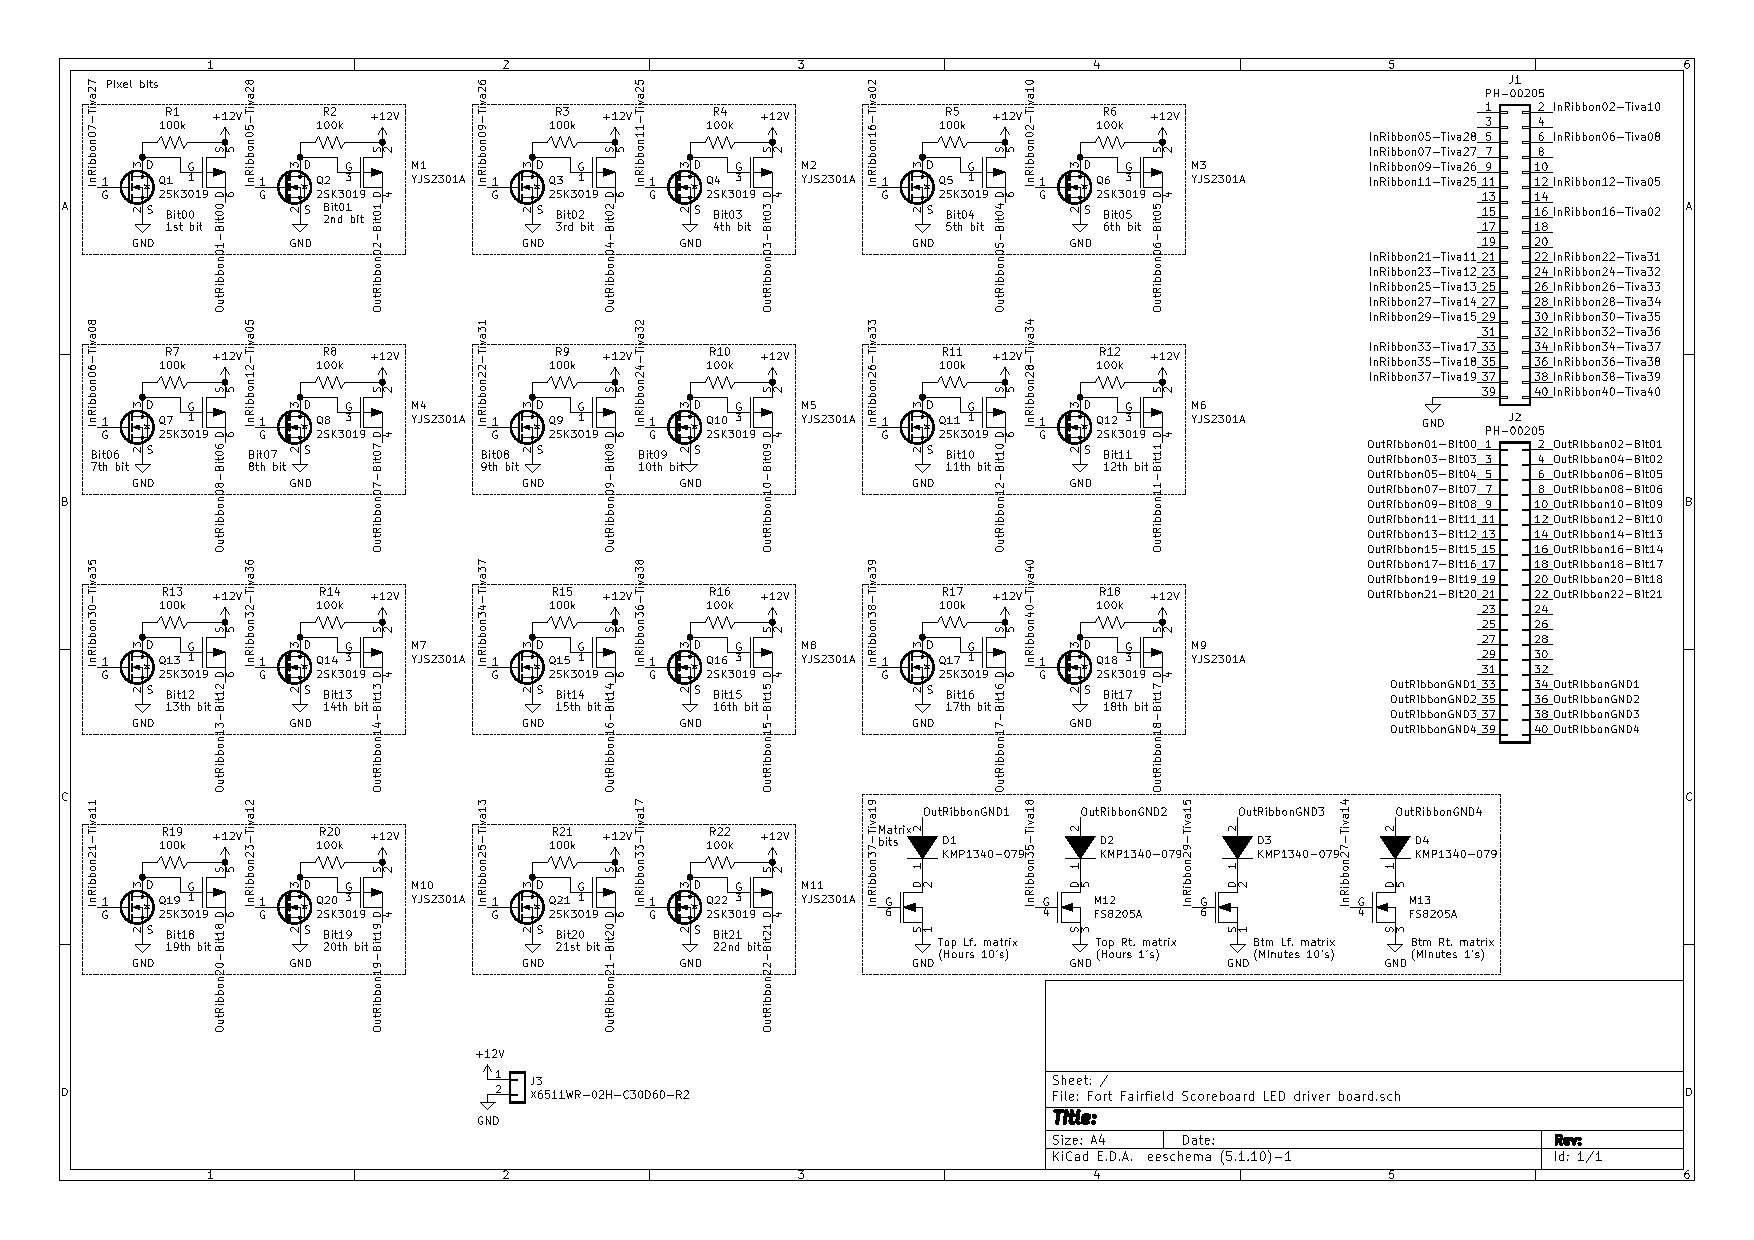
\includepdf[pages=-,scale=0.85,angle=90]{evidence_createSchematics_1_LEDMuxer.pdf}
  \rotcaption{Schematic of LED Multiplexing PCB}
\end{figure}


\newpage
\newpage

\section{Data Sheets}
\label{appendix:datasheets}
\titlespacing*{\chapter}{0pt}{0pt}{-40pt}
\begin{figure}[htp]
    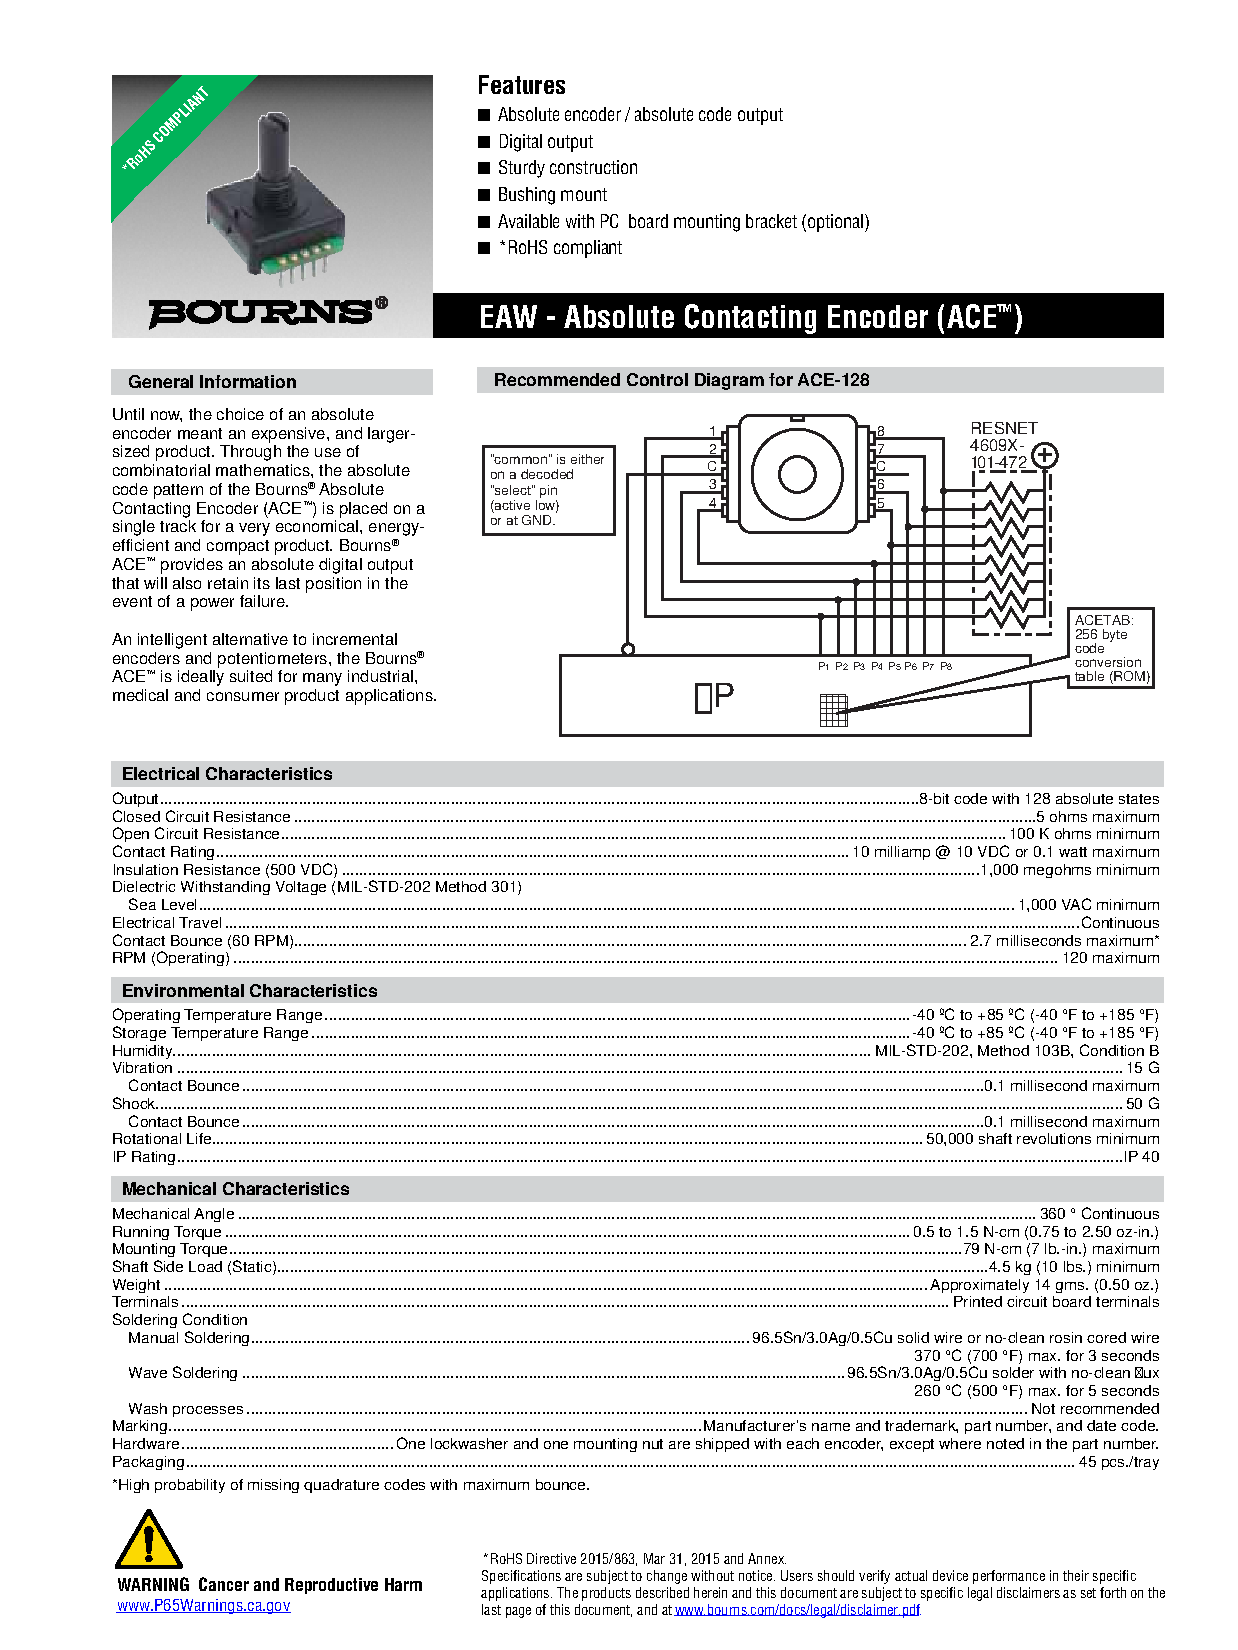
\includepdf[pages=-,scale=.85]{encoderDataSheet.pdf}
    \newpage
\end{figure}
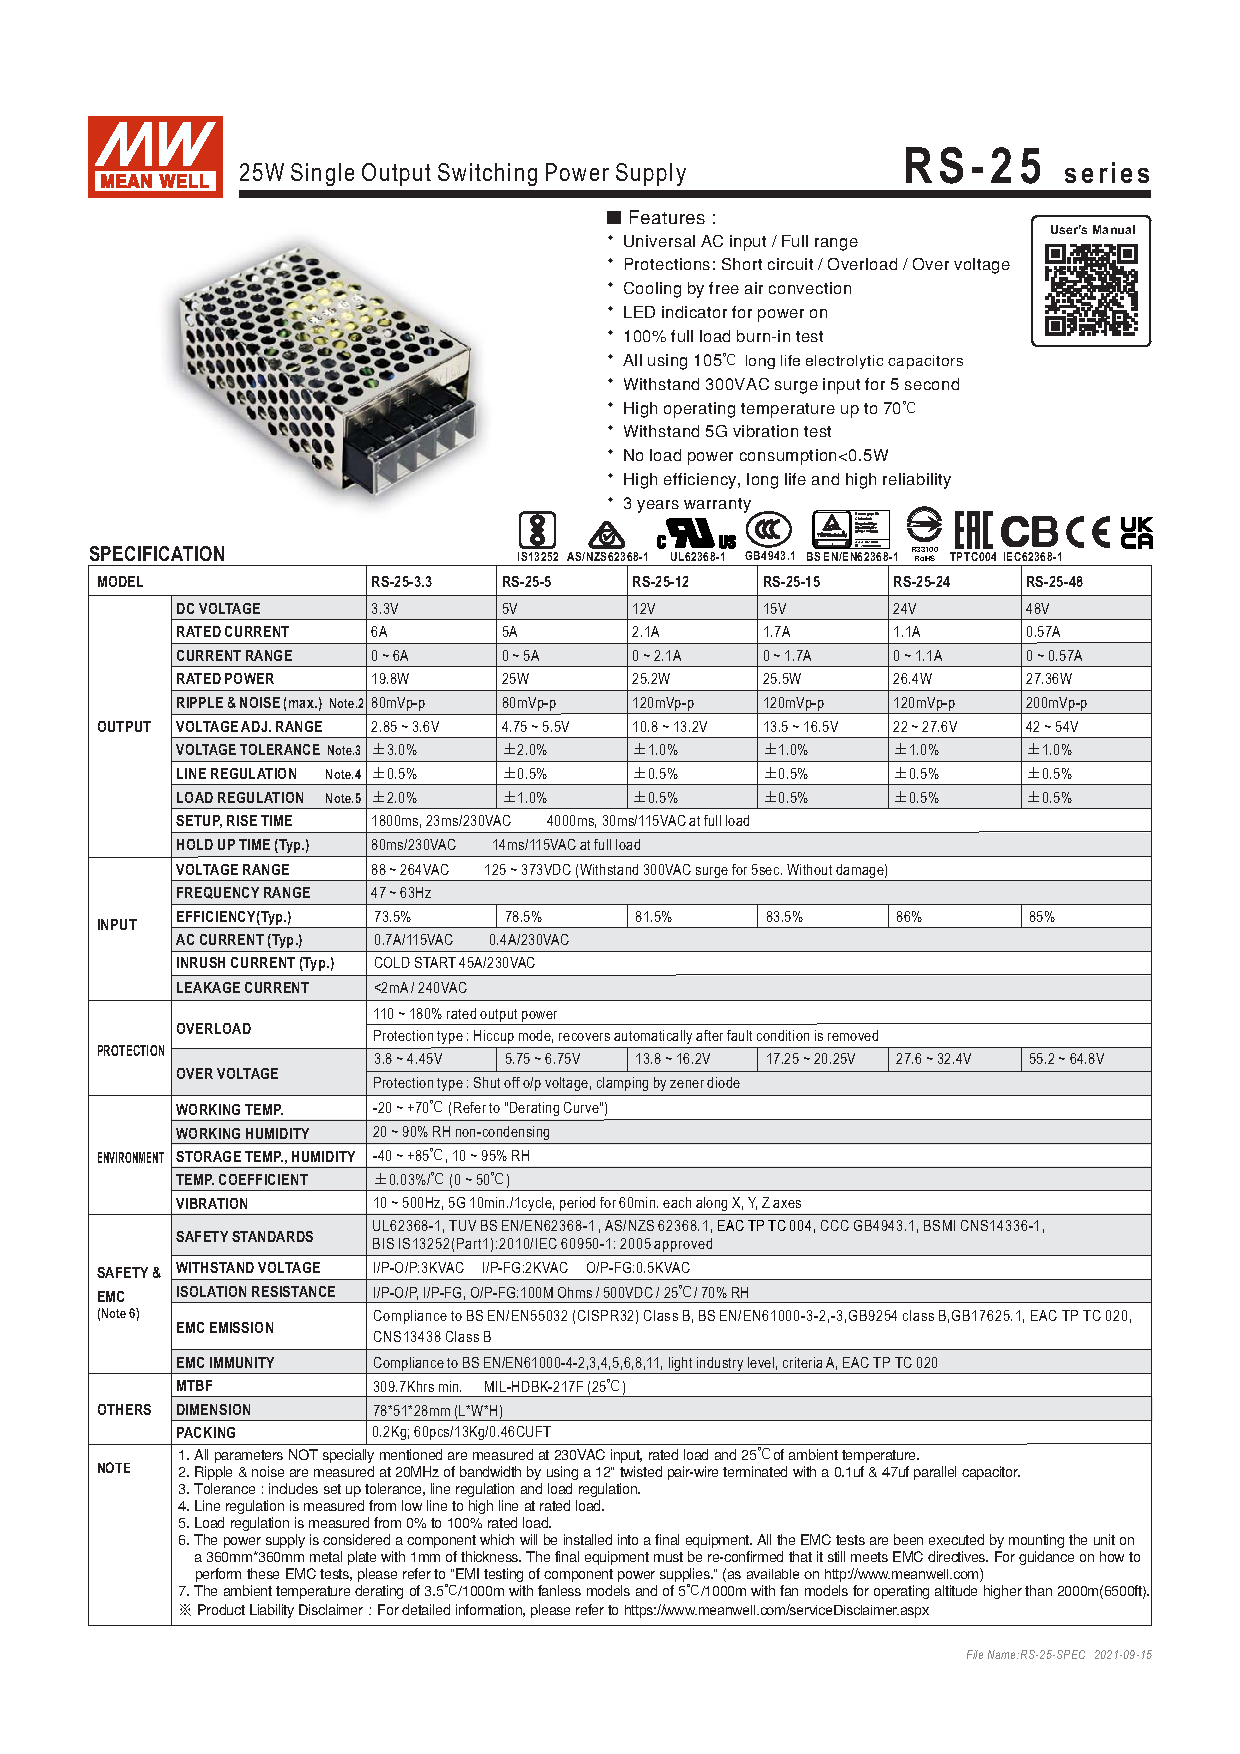
\includepdf[pages=-,scale=1]{meanwellDatasheet.pdf}
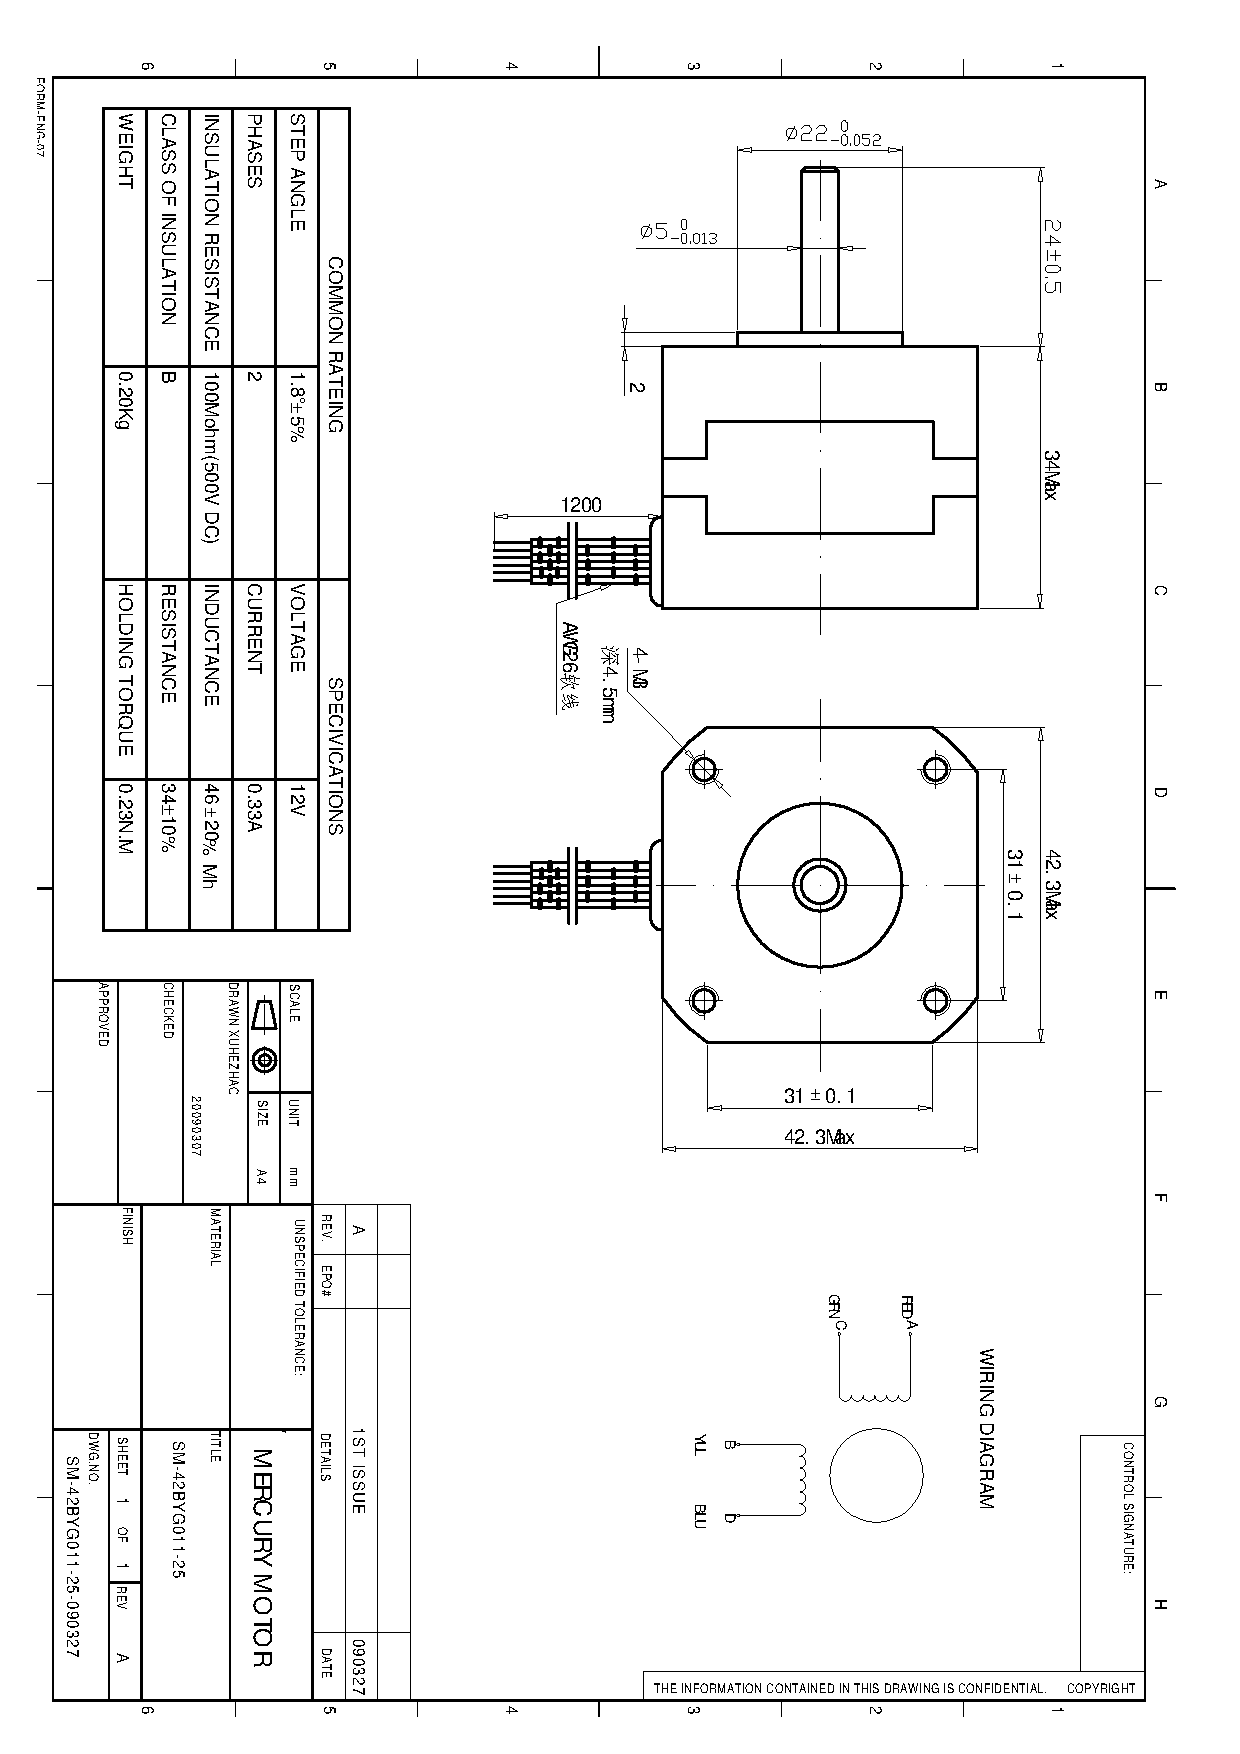
\includepdf[pages=-,scale=1]{MotorDatasheet_rot_pdftkonly.pdf}
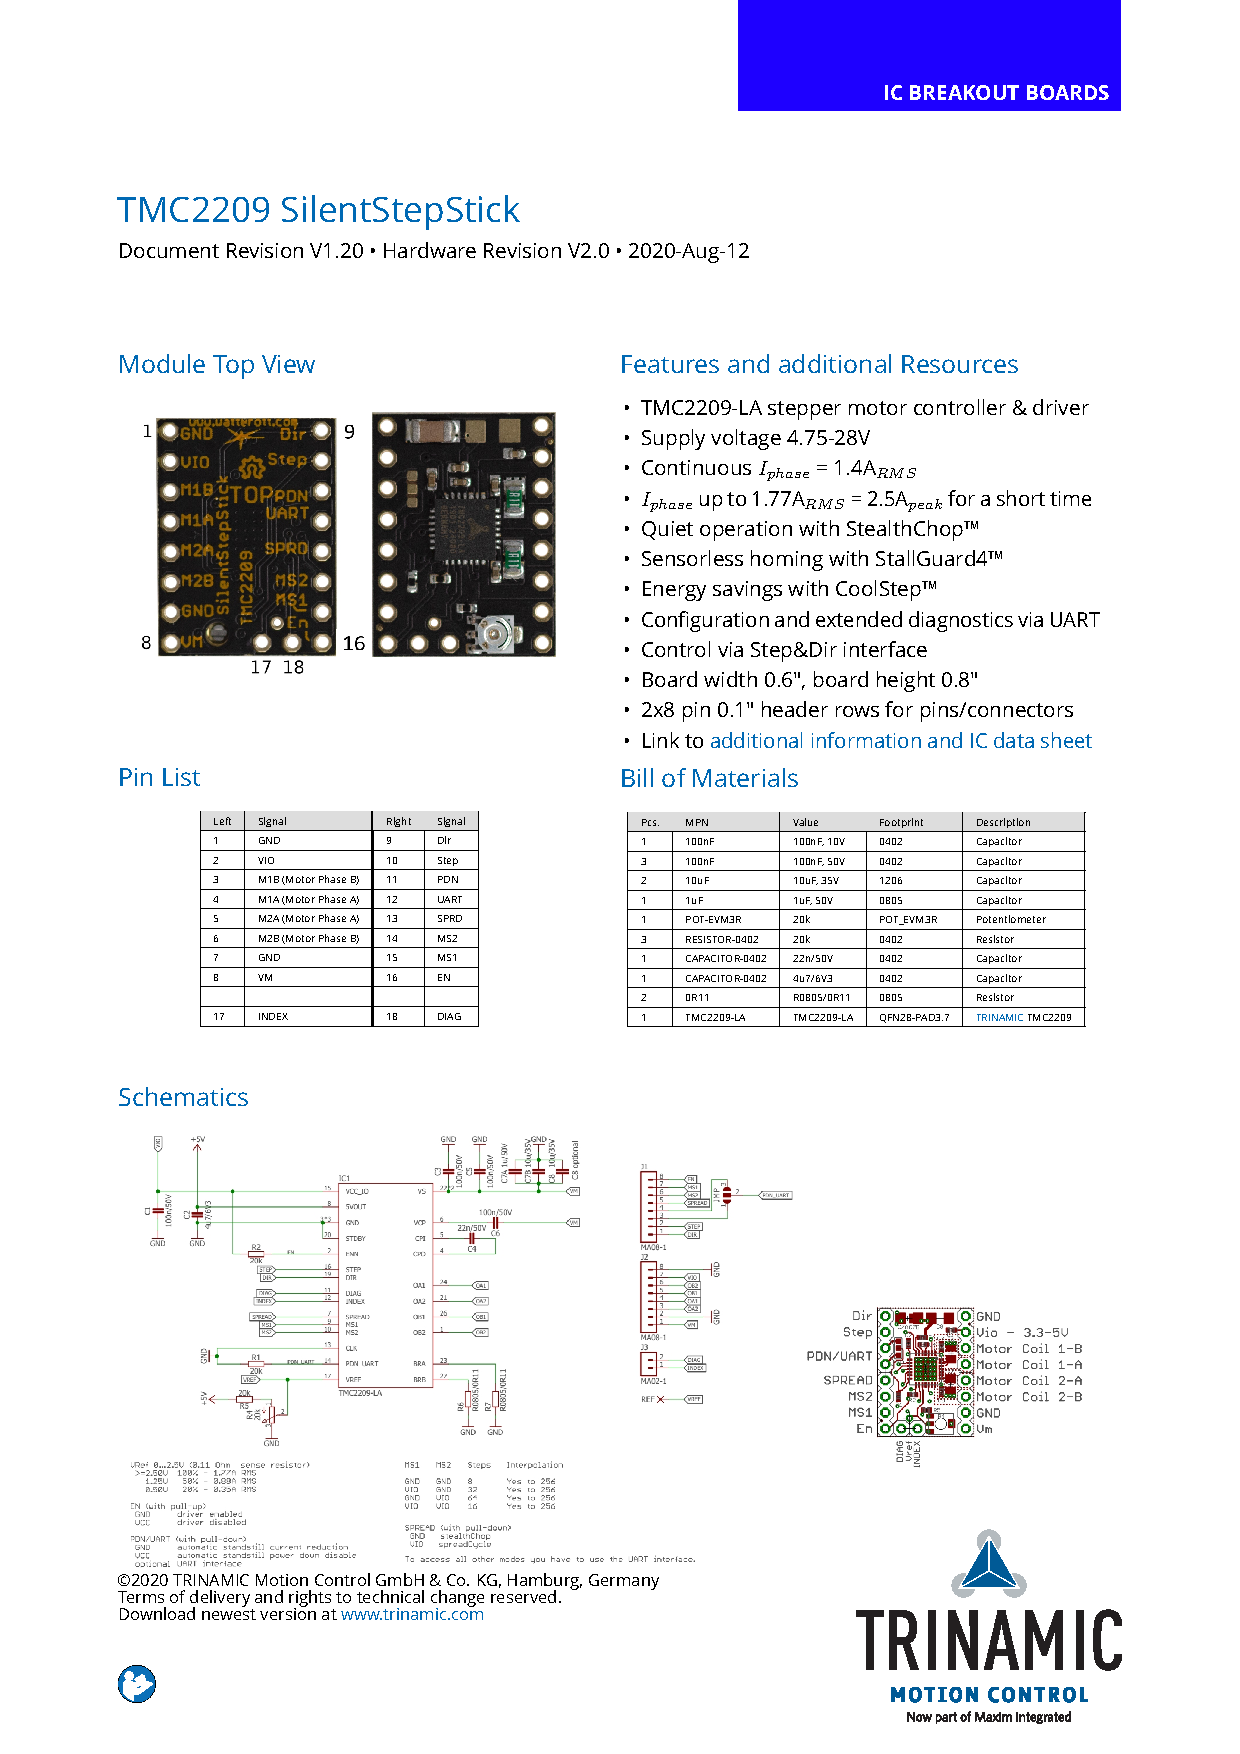
\includepdf[pages=-,scale=1]{TMC2209DataSheet.pdf}
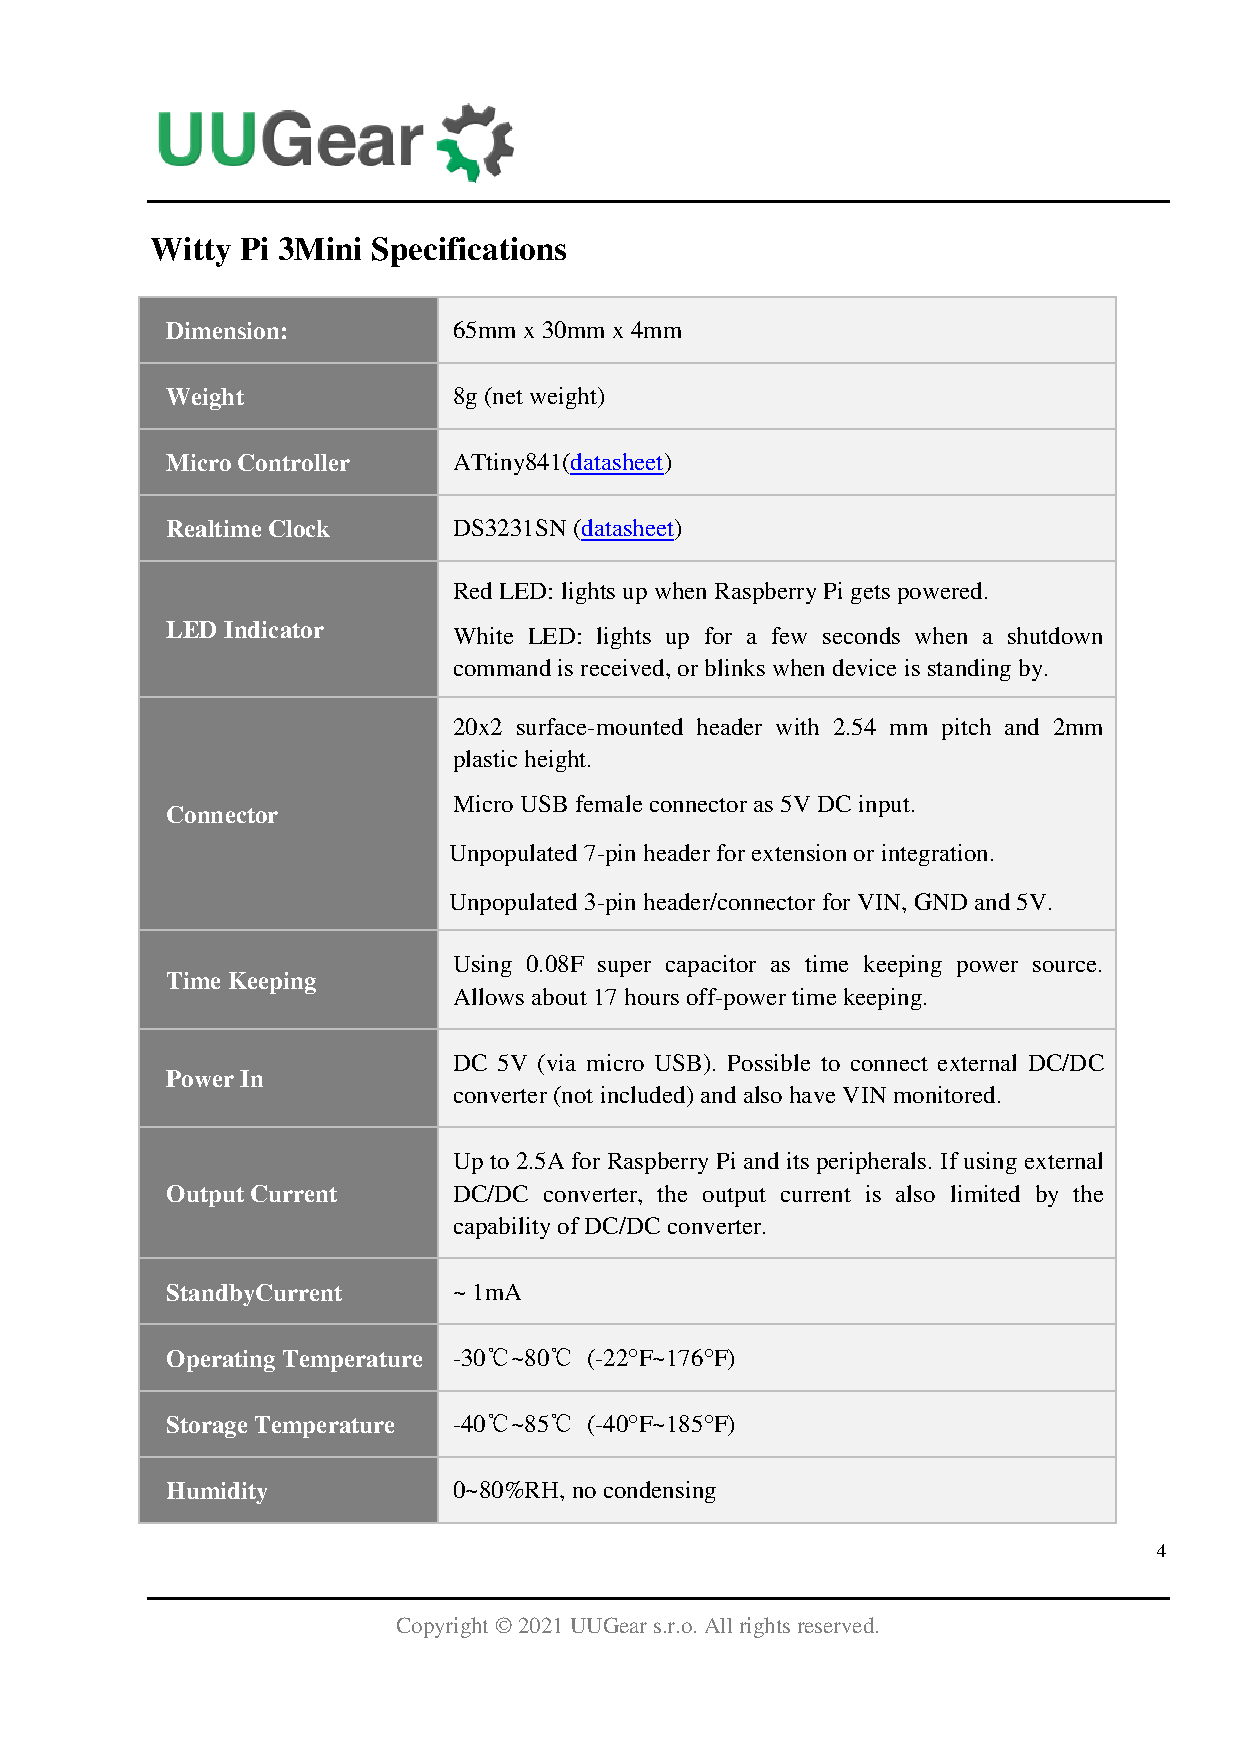
\includepdf[pages=-,scale=1]{WittyDataSheet.pdf}

\newpage

%add later, rn self explanatory
%\section{Operating Instructions}
%\label{appendix:instruct}

\end{document}
